% ----------------------- TODO ---------------------------
% Diese Daten müssen pro Blatt angepasst werden:
\newcommand{\NUMBER}{1}
\newcommand{\EXERCISES}{5}
% Diese Daten müssen einmalig pro Vorlesung angepasst werden:
\newcommand{\COURSE}{Project - CUDA-Aware MPI}

\newcommand{\STUDENTA}{Zirong Cai}
\newcommand{\STUDENTB}{Phuong Nguyen}
\title{\vspace{-2em} Final Project - CUDA-Aware MPI\vspace{-0.5em}}
\author{ \STUDENTA, \STUDENTB}
\date{\today {\vspace{-1cm}}}

% ----------------------- TODO ---------------------------

\documentclass[article]{scrartcl}

\usepackage[utf8]{inputenc}
\usepackage[english]{babel}
\usepackage{amsmath}
\usepackage{amssymb}
\usepackage{fancyhdr}
\usepackage{color}
\usepackage{graphicx}
\usepackage{lastpage}
\usepackage{listings}
\usepackage{tikz}
\usepackage{pdflscape}
\usepackage{float}
\usepackage{polynom}
\usepackage{hyperref}
\usepackage{tabularx}
\usepackage{forloop}
\usepackage{geometry}
\usepackage{listings}
\usepackage{caption}
\usepackage{subcaption}
%\usepackage{subfigure}
\usepackage{fancybox}
\usepackage{tikz}
\usepackage{algpseudocode,algorithm,algorithmicx}
%\usepackage{biblatex}
\usepackage{cite}

\setkomafont{title}{\normalsize}
\setkomafont{author}{\small}
\setkomafont{date}{\small}
\setkomafont{section}{\normalfont \normalsize \textbf}
\setkomafont{subsection}{\normalfont}
\renewcommand*{\thesubsection}{\alph{subsection}}

\setkomafont{subsubsection}{\normalfont\itshape}

%\lstset { %
%    language=C++,
%    backgroundcolor=\color{black!5}, % set backgroundcolor
%    basicstyle=\footnotesize,% basic font setting
%}
	\lstset{language=C++,
	basicstyle=\ttfamily\footnotesize,
	keywordstyle=\color{blue}\ttfamily,
	stringstyle=\color{red}\ttfamily,
	commentstyle=\color{green}\ttfamily,
	morecomment=[l][\color{magenta}]{\#}
}
%\captionsetup[lstlisting]{ format=listings, labelfont=white, textfont=white}

%Größe der Ränder setzen
\geometry{a4paper,left=3cm, right=3cm, top=3cm, bottom=3cm}

%Kopf- und Fußzeile
\pagestyle {fancy}\usepackage{listings}
\fancyhead[L]{\STUDENTA, \STUDENTB}
\fancyhead[R]{\COURSE}

\fancyfoot[L]{}
\fancyfoot[R]{Page \thepage /\pageref*{LastPage}}

\begin{document}


\maketitle
\thispagestyle{fancy}

\section{Git Repository}

\href{https://gitlab.lrz.de/phuongng_tum/hpclab}{Click here } or find the link in \cite{gitrepo}.
\section{Motivation}
\subsection{SWE Code with CUDA - the current state}
%- 1 paragraph for CUDA-Aware MPI.

%- 1 paragraph SWE: lists 2 functions that are dominant in runtime and which we implemented CUDA-Aware MPI.  

In the original code, the CUDA and MPI were implemented which allow us to run the simulation with multiple GPUs. However, there exist some disadvantage as follows:
\begin{itemize}
	\item First, each data set has two copies, one locates on the \textit{host} (which is CPU), the other locates on the \textit{devices} (which are GPUs). Prior to the computation on GPUs, one always need to copy the data from host to device, and back after the computation. This way of implementation is not very easy and obvious for programmers, causing extra efforts for coding and debugging.
	\item Second, it's common in scientific simulation that MPI processes need to communicate during the computation time. With the original CUDA implementation, the calculation part is done on the GPUs, thus the updated data is located on GPUs. For inter-processes communication, one needs to copy data from GPUs back to CPUs, then call the MPI routines for exchanging data, and then copy data back to GPUs again. This requires extra efforts for programming, at the same time not very efficient.
\end{itemize}
\begin{figure}[htpb]
	\centering
	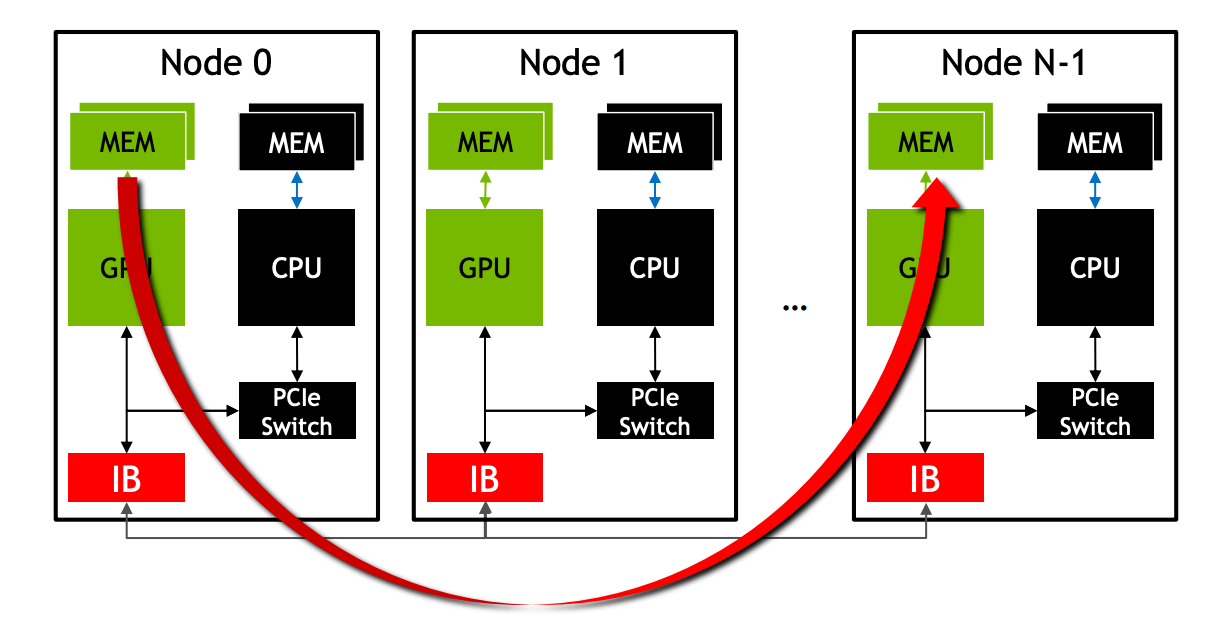
\includegraphics[width=.8\textwidth,height=.8\textheight,keepaspectratio=true]{../figs/mpi+cuda.png}
	\caption{MPI+CUDA Model}
	\label{fig:mpi+cuda}
\end{figure}
\subsection{Motivations to implement CUDA-Aware MPI}
We are looking for a way to have more efficient CUDA + MPI code, especially the communication part. Fortunately, the current modern hardware and vendor software has additional support for this, through for example GPUDirect RDMA or GPUDirect P2P, which allows communication between GPUs directly, bypassing host (CPUs). In order to utilize this state-of-the-art advantages, we implemented CUDA-Aware MPI for the SWE code, which also involves the work of implementing Virtual Unified Memory.


\section{Theoretical Background}


\subsection{Virtual Unified Memory}


%The original project uses MPI to assign tasks to different processors.
%Each processor then copies the corresponding data to GPU and use GPU to compute the result independently.
%After the computation is done, the result will be copied back to CPU and again use MPI to propagate the result to other processes.

According to \cite{unifiedMemory}, Unified Memory is a single memory address space accessible from any processor in a system. 
This hardware/software technology allows applications to allocate data that can be read or written from code running on either CPUs or GPUs. 
When code running on a CPU or GPU accesses data allocated this way (often called CUDA managed data), 
the CUDA system software and/or the hardware takes care of migrating memory pages to the memory of the accessing processor.
In other words, we can assume that GPU and CPU are using the same memory space.(see \ref{fig:UnifiedMemory})
% \subsection{CUDA-Aware MPI}
% The overhead of transmitting data in this way may be too high. A way to eliminate such overhead is directly transmitting data from one GPU node to another GPU node, which is called CUDA-AWARE-MPI(see \ref{fig:mpi+cuda} ).
\begin{figure}[htpb]
	\centering
	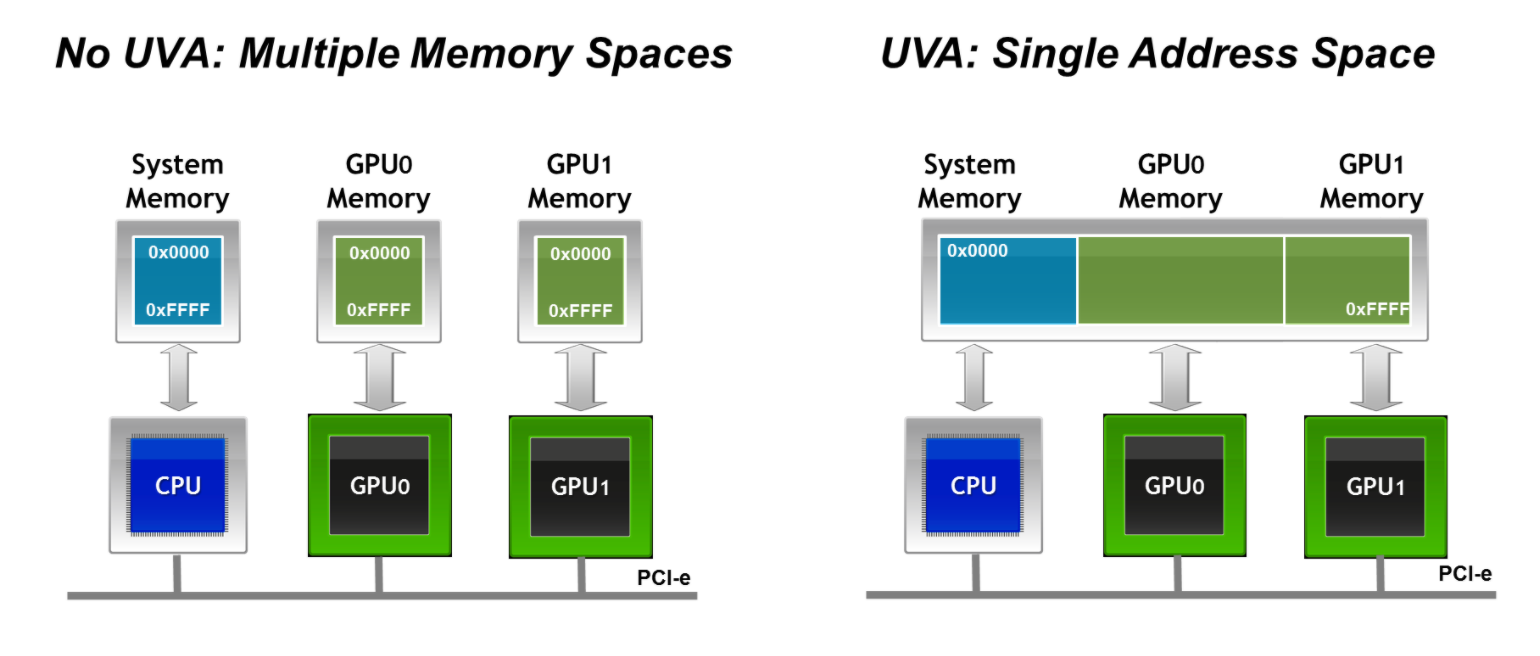
\includegraphics[width=\textwidth,keepaspectratio=true]{../figs/UnifiedMemoryCompare.png}
	\caption{No Unified Memory Vs. Unified Memory\cite{introCudaAware}}
	\label{fig:UnifiedMemory}
\end{figure}

% In order to turn our project into CUDA-AWARE-MPI, we need a technology called Unified Memory.
\subsection{NVIDIA GPUDirect}
NVIDIA GPUDirect technologies provide high-bandwidth, low-latency communications with NVIDIA GPUs. 
GPUDirect for accelerated communication with network and storage devices was the first GPUDirect technology. This feature allows the network fabric driver and the CUDA driver to share a common pinned buffer in order to avoids an unnecessary memcpy within host memory between the intermediate pinned buffers of the CUDA driver and the network fabric buffer\ref{fig:GPUDirect}.
\begin{figure}[htpb]
	\centering
	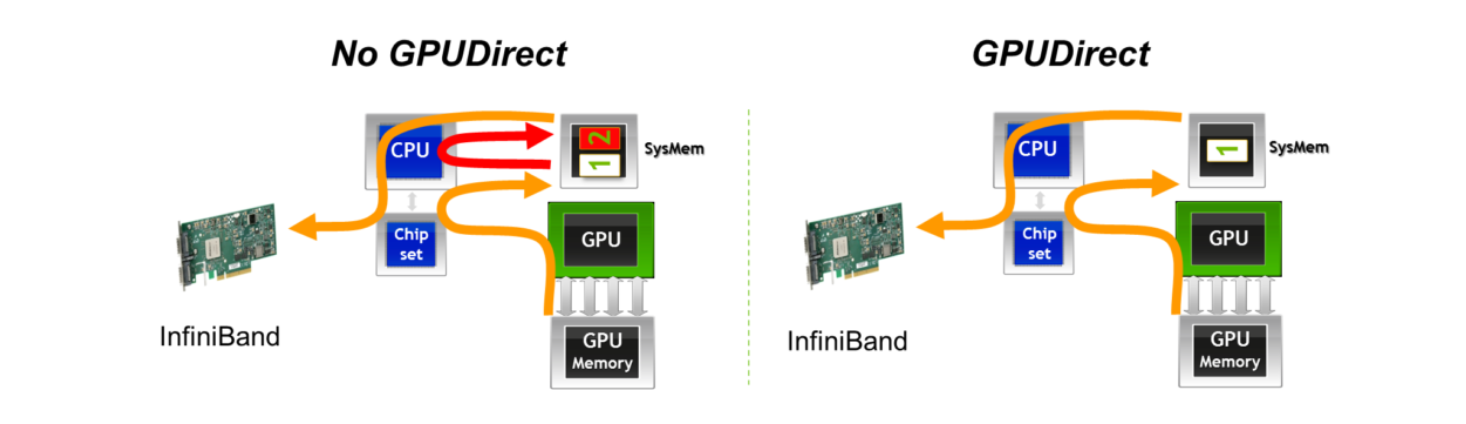
\includegraphics[width=\textwidth,keepaspectratio=true]{../figs/GPUDIrect.png}
	\caption{No GPUDirect Vs. GPUDirect\cite{introCudaAware}}
	\label{fig:GPUDirect}
\end{figure}


Another variant is GPUDirect for Peer-to-Peer (P2P) transfers, which was introduced with CUDA 4.0 and can accelerate intra-node communication. Buffers can be directly copied between the memories of two GPUs in the same system with GPUDirect P2P.(\ref{fig:GPUDirectP2P})
\begin{figure}[htpb]
	\centering
	\includegraphics[width=\textwidth,keepaspectratio=true]{../figs/GPUDIrectP2P.png}
	\caption{No GPUDirect P2P Vs. GPUDirect P2P\cite{introCudaAware}}
	\label{fig:GPUDirectP2P}
\end{figure}

The third feature, also the newest, is support for Remote Direct Memory Access (RDMA), with which buffers can be directly sent from the GPU memory to a network adapter without staging through host memory.(\ref{fig:GPUDirectRDMA})
\begin{figure}[htpb]
	\centering
	\includegraphics[width=\textwidth,keepaspectratio=true]{../figs/GPUDIrectRDMA.png}
	\caption{No GPUDirect RDMA Vs. GPUDirect RDMA\cite{introCudaAware}}
	\label{fig:GPUDirectRDMA}
\end{figure}

\subsection{CUDA-Aware MPI}
There are several commercial and open-source CUDA-aware MPI implementations available:
\begin{itemize}
	\item MVAPICH2
	\item OpenMPI
	\item IBM Platform MPI 
\end{itemize}
There are many reasons for wanting to combine the two parallel programming approaches of MPI and CUDA. A common reason is to enable solving problems with a data size too large to fit into the memory of a single GPU, or that would require an unreasonably long compute time on a single node. Another reason is to accelerate an existing MPI application with GPUs or to enable an existing single-node multi-GPU application to scale across multiple nodes. With CUDA-aware MPI these goals can be achieved easily and efficiently.
CUDA-aware MPI not only makes it easier to work with a CUDA+MPI application, it also makes the application run more efficiently for two reasons:
\begin{itemize}
	\item All operations that are required to carry out the message transfer can be pipelined;
	\item Acceleration technologies like GPUDirect can be utilized by the MPI library transparently to the user.
\end{itemize}
\section{Implementation}
\subsection{Automated Regression Test}
The automation test implementation including:
\begin{itemize}
	\item \textit{src/examples/swe\_test.cpp}: a test program which prints \textit{WaterHeight} to a output file.
	\item \textit{test/error\_check.py}: a script which calculates the absolute difference between 2 sets of input data.
	\item \textit{test/run\_test.sh}: an executable script which first compiles the needed binaries, then runs the tests, and check for errors. 
\end{itemize}
We have implemented a test program in \textit{swe\_test.cpp} which based on \textit{swe\_mpi.cpp}. The main simulation, including initialization and time integration, is kept the same as in the \textit{swe\_mpi.cpp}, but without writing outputs out. In addition to the simulation, we implemented in \textit{swe\_test.cpp} a parallel outputting which can write the \textit{WaterHeight} to a output file. The implement of parallel outputting is as follow:
\begin{frame}[]
	%\frametitle{Inserting source code}
	\lstset{language=C++,
		basicstyle=\ttfamily\footnotesize,
		keywordstyle=\color{blue}\ttfamily,
		stringstyle=\color{red}\ttfamily,
		commentstyle=\color{green}\ttfamily,
		morecomment=[l][\color{magenta}]{\#}
	}
\begin{lstlisting}[frame=single]
Float2D h_test(l_waveBlock->getWaterHeight(), false);
 // 2D subarray Datatype for MPI_File_set_view
int ndims = 2;  
int gsizes[2], lsizes[2], starts[2];
gsizes[0] = l_nX;
gsizes[1] = l_nY;
lsizes[0] = l_nXNormal;
lsizes[1] = l_nYNormal;
starts[0] = l_blockPositionX * l_nXNormal;
starts[1] = l_blockPositionY * l_nYNormal;
MPI_Datatype subarr_type;
MPI_Type_create_subarray(ndims,  gsizes, lsizes, starts, \ 
			MPI_ORDER_C, MPI_FLOAT, &subarr_type);
MPI_Type_commit(&subarr_type);

// Datatype to exclude ghostcell values
MPI_Datatype print_type;
MPI_Type_vector(l_nXLocal, l_nYLocal, l_nYLocal + 2, MPI_FLOAT, &print_type);
MPI_Type_commit(&print_type);

MPI_File file;
MPI_Status status;
std::string filename("WaterHeight_" + \
			std::to_string(l_numberOfProcesses) + "mpi.txt");
MPI_File_open(MPI_COMM_WORLD, filename.c_str(), MPI_MODE_WRONLY + \
			MPI_MODE_CREATE, MPI_INFO_NULL, &file);

MPI_File_set_view(file, 0, MPI_FLOAT, subarr_type, "native", MPI_INFO_NULL);
MPI_File_write_all(file, &h_test[1][1], 1, print_type, &status);

MPI_File_close(&file);
\end{lstlisting}
\end{frame}

The resultting output files from the MPI Parallel IO are raw data files which are not human-readable. We need to have a additional step to post-processing this data file so that the python script - \textit{error\_check.py} - can read it. For that we use:
\begin{lstlisting}
$ od -v -An -f WaterHeight_Xmpi.txt | tr '\n' ' '
\end{lstlisting}
After that, we use \textit{error\_check.py} script to check for the error. This script can calculate the absolute element-by-element difference between any two data set, which their file name are passed to the command line as arguments as follow:
\begin{lstlisting}
$ python3 error_check.py dataset1.txt dataset2.txt
\end{lstlisting}

In short, for a automation test, one can execute the script \textit{test/run\_test.sh} on the GPU node (x-wing0). The script will first check if the needed binaries are present and compile those binaries in case they are not. Then it will run all defined tests with 1 MPI and 4 MPI processes, including test the pure MPI implementation, the MPI + CUDA implementation, and the MPI + CUDA-Aware MPI implementation.

\subsection{GPU script}
For this project, it is essential to be able to map more than 1 MPI processes to more than 1 GPUs. For this, we created a script called \textit{gpu\_bind.sh} which map each MPI process to according GPU Devices. The script is as follow:
\begin{lstlisting}[frame=single, label={gpu_script}]
#!/bin/bash
export CUDA_VISIBLE_DEVICES=$OMPI_COMM_WORLD_LOCAL_RANK
case $OMPI_COMM_WORLD_LOCAL_RANK in
[0]) cpus=0;;
[1]) cpus=1;;
[2]) cpus=2;;
[3]) cpus=3;;
esac
numactl --physcpubind=$cpus $@
\end{lstlisting}
The command to run the simulation with multiple GPUs is as follow:
\begin{lstlisting}
mpirun -np 4 ../gpu_bind.sh ./swe-cuda -x ${NX} -y ${NY} -c ${STEPS} -o .
\end{lstlisting}

\subsection{Unified Memory}
As time goes by, CUDA programming has gotten easier. Back to 10 years ago, since GPU and CPU use their own memory independently,
we as a CUDA programmer need to explicitly define how the data should be transmitted between CPU and GPU. 
It's okay when we only need GPU for pure computation and then get a result from it. But in our program, we not only need to process the data arrays
in GPU to update the wave, but also need the data in CPU for MPI communication. Now with unified memory,
we are able to define an array and use it everywhere without doing explicitly data transmition.
Following is how it is implemented in our code:

\begin{lstlisting}[frame=single]
Float2D(int _cols, int _rows, bool _allocateMemory = true):
rows(_rows),
cols(_cols),
allocateMemory(_allocateMemory) {
if (_allocateMemory) {
  #if defined(CUDA_AWARE_MPI) 
  cudaMallocManaged((void**)&elem, rows*cols*sizeof(float)); 
  #else 
  elem = new float[rows*cols];
  #endif
}
}
\end{lstlisting}
And with this, we have decided to allocate \textit{h}, \textit{hv}, \textit{hu} with virtual unified memory address since we need to have access to these data from both host and devices. For other helper data which is used only in the \textit{\_device\_} functions, we still allocate it on the usual device memory with \textit{cudaMalloc}. \\
Since \textit{h}, \textit{hv}, \textit{hu} are "shared" pointers which can be access by both hosts and devices, we passed \textit{h}, \textit{hv}, \textit{hu} into all related kernel functions instead of \textit{hd}, \textit{hvd}, \textit{hud}. Besides, all explicit copy between Host and Device are not needed anymore, thus they were removed.

\subsection{MPI Communication \& Ghost Layer Implementation}
\label{mpi_datatype}

As mentioned above, with unified memory, we can use the data array just like a normal in CPU-allocated array. Thus, for MPI communication, we simply can pass the pointer of data which lie on unified memory to the MPI Routines. The MPI deamon of CUDA-Aware MPI (here is OpenMPI) can handle the rest of the procedure, such as it will look for the location of the data and then pack the data. Thus, for ghost layer exchanges, we can send data directly from the data grid, without addition packing. Then the \textit{MPI\_Type\_Vector} for \textit{rows} would be similar to the case when we have pure MPI implement (without CUDA) rather then the one of CUDA implementation. In mean if we want to send the row 1 of the data grid, since we have column-wise format, the address of elements in the row will look like: \textit{1, 1 + nRows, 1+2*nRows, \dots} where \textit{nRows} is total number of rows in the grid. \\
We defined the \textit{MPI\_Type\_vector} as follows:
\begin{lstlisting}[frame=single]
  MPI_Datatype l_mpiRow;
  MPI_Type_vector(l_nXLocal + 2, 1, l_nYLocal + 2, MPI_FLOAT, &l_mpiRow);
\end{lstlisting}

\subsection{Fixing the original CUDA implementation}
\label{fixing_bugs}
We have tested the original CUDA implementation with 4 GPUs and the results were surpringly incorrect (see Figure~\ref{figs:validation_cuda}). We investigated further on this and found out a few issues:


Bug 1: In the \textit{SWE\_WavePropagationBlockCuda::updateUnknowns()}, there is a macro function to check if \textit{USEMPI} is defined then call a function \textit{synchCopyLayerBeforeRead}, but the \textit{USEMPI} is not defined anywhere else. The purpose of \textit{synchCopyLayerBeforeRead} is to copy data (h, hv, hu) from Device to Host, in preparation for ghost layer exchanging with neighbors, thus especially important when we have multi GPUs. We suggest to update the code with the patch at Listing~\ref{patch1}.

\lstinputlisting[frame=single,language=bash,caption={Patch file for CMakeLists.txt}, captionpos=b, label={patch1}]{../SWE/cmake.diff}

Bug 2: After we called for \textit{exchangeGhostLayer} functions in the main code, we call \textit{setGhostLayer()} which calls \textit{setBoundaryConditions()} where all received data from neighbors are copied to according columns/rows on the device memory. However, when the BOUNDARY is TOP or BOTTOM, it copies data from bottomLayerDevice/topLayerDevice to respective rows, but the data received from neighbors are still in bottomLayer/topLayer and has not moved to Device so far. Thus we suggest to have the patch at Listing~\ref{patch2} to fix this issue.
\lstinputlisting[frame=single,language=bash,caption={Patch file for SWE\_BlockCUDA.cu},captionpos=b, label={patch2}]{../SWE/src.diff}


\section{Results and Discussion}
\subsection{Validation}
\subsubsection{Validation of the GPU script}
With the script at Listing~\ref{gpu_script}, we are able to involve more than 1 GPUs in the simulation. The Figure~\ref{fig:GPUMonitor} shown the GPU monitoring when we ran the test with 4 GPUs on the testing node.
\begin{figure}[htpb]
	\centering
	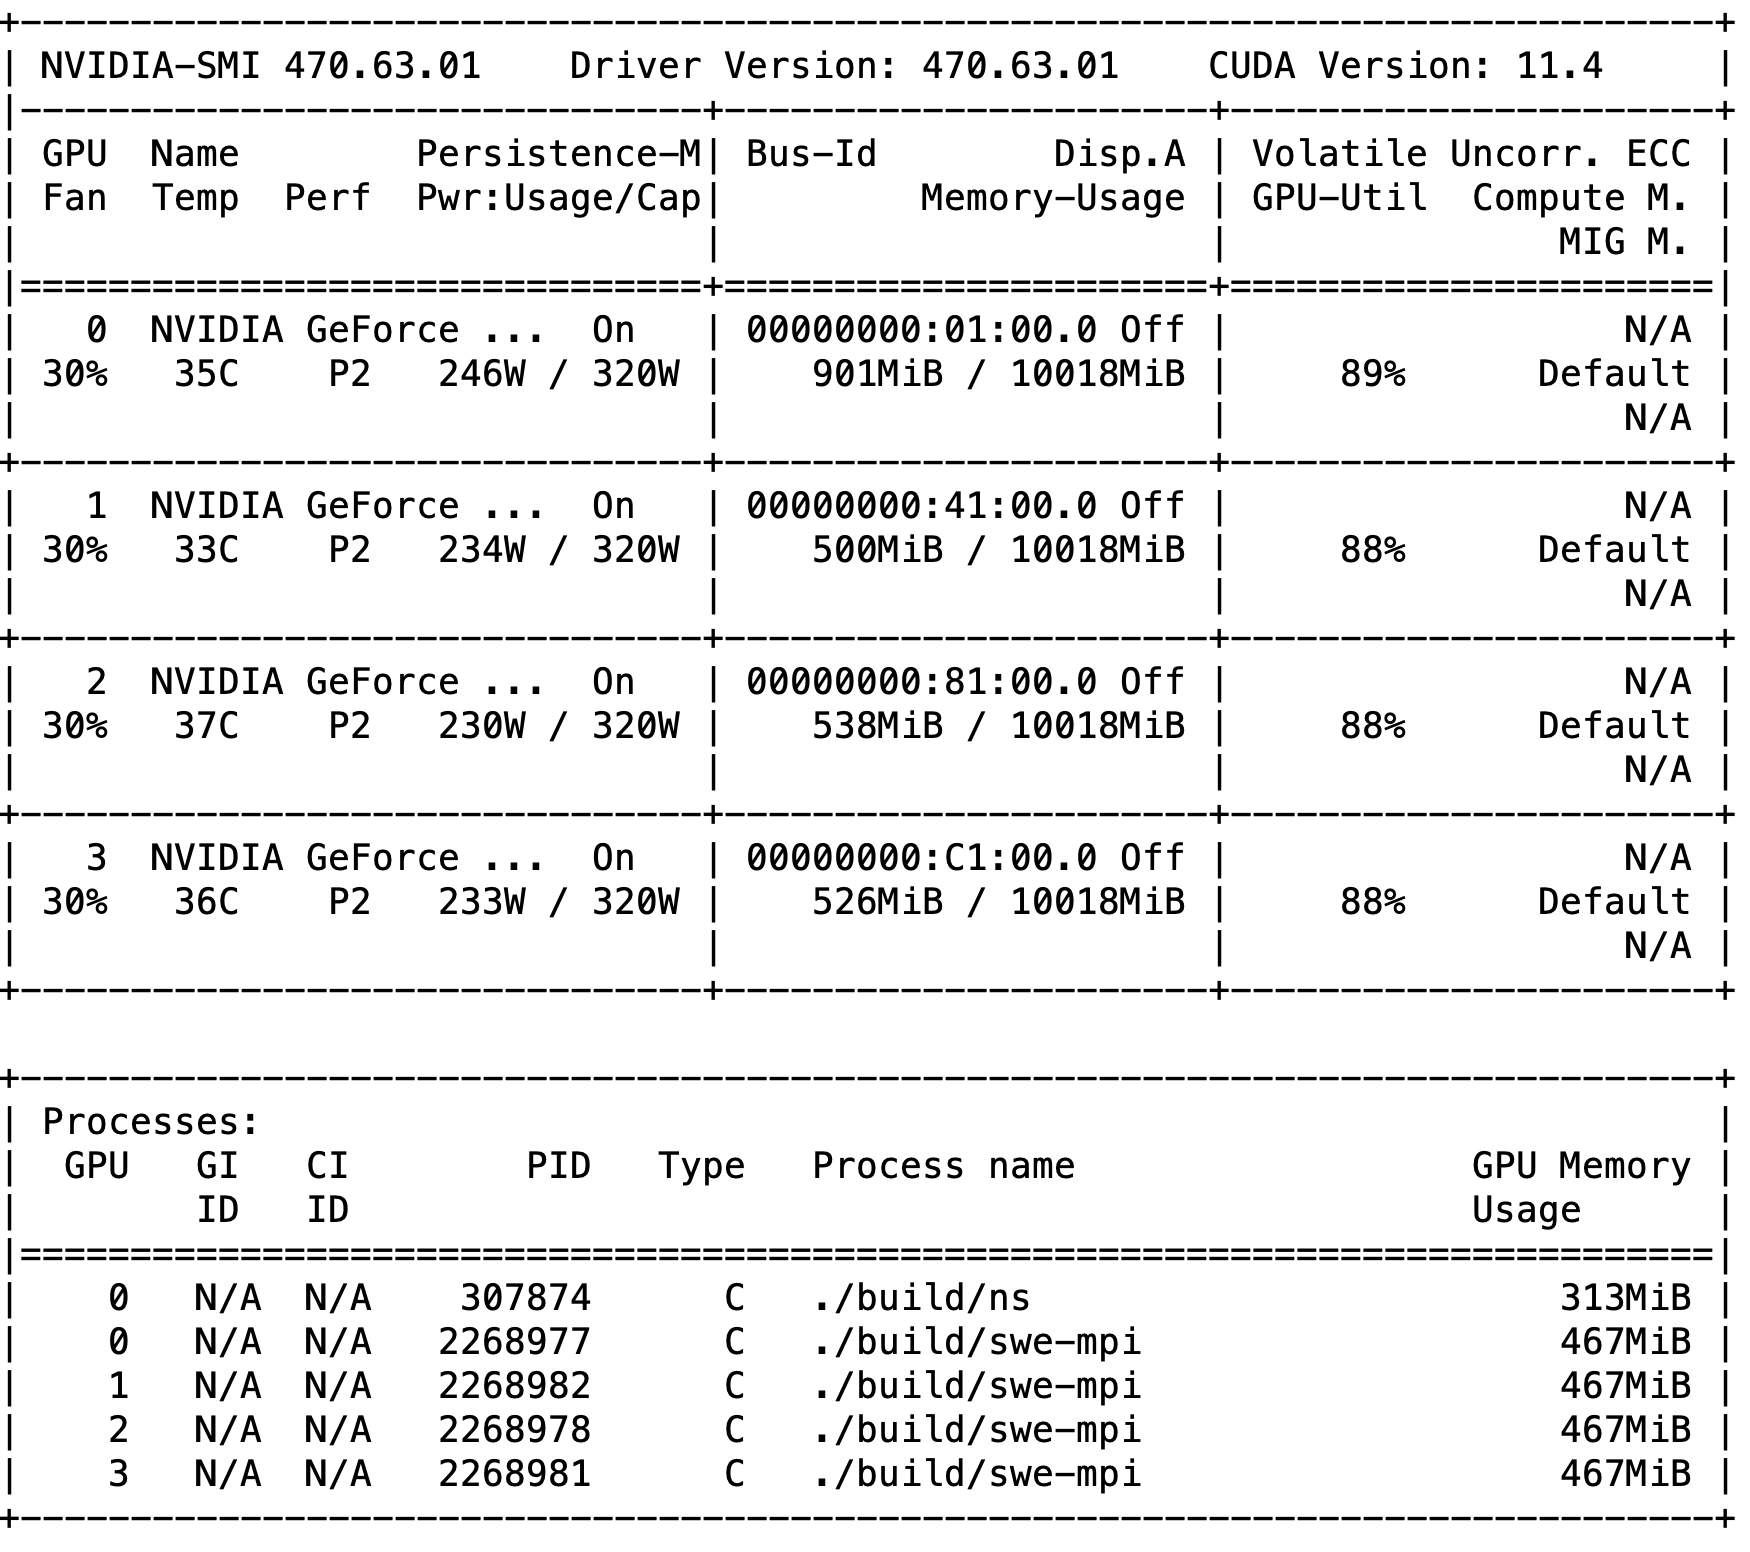
\includegraphics[width=0.7\textwidth,keepaspectratio=true]{../figs/cuda4096-4.png}
	\caption{GPU Monitoring}
	\label{fig:GPUMonitor}
\end{figure}
\subsubsection{Validation of the fixed CUDA implementation}
From Figure~\ref{figs:validation_cuda} we see that the original MPI+CUDA version with 4 MPI processes does not give us the same output as the MPI only version with 1 MPI process. And this is further proven by our test script. Table \ref{table:cuda} shows the absolute difference of the array WaterHeight between different the two versions, where \textit{1 mpi} means 1 MPI process with the pure MPI version, the same for \textit{4 mpi}, while it's 4 MPI processes with 4 GPUs for the case of \textit{4 cuda}. With the patches we suggested in section~\ref{fixing_bugs}, the error of the \textit{4 cuda} in comparision with \textit{1 mpi} is acceptable now. There is still a small error which propagates from \textit{1 mpi} - \textit{1 cuda}. Besides, when we run the same test multiple times, the error values between \textit{1 mpi} - \textit{4 mpi} are not consistent. Thus, there are still bugs in the pure MPI implementation and pure CUDA implementation. However, this is our of the scope of our project, since we did not touch the implementation of the original MPI version nor the way the main CUDA kernel. 
\begin{figure}[htpb]
    \centering
    \begin{subfigure}{.3\textwidth}
        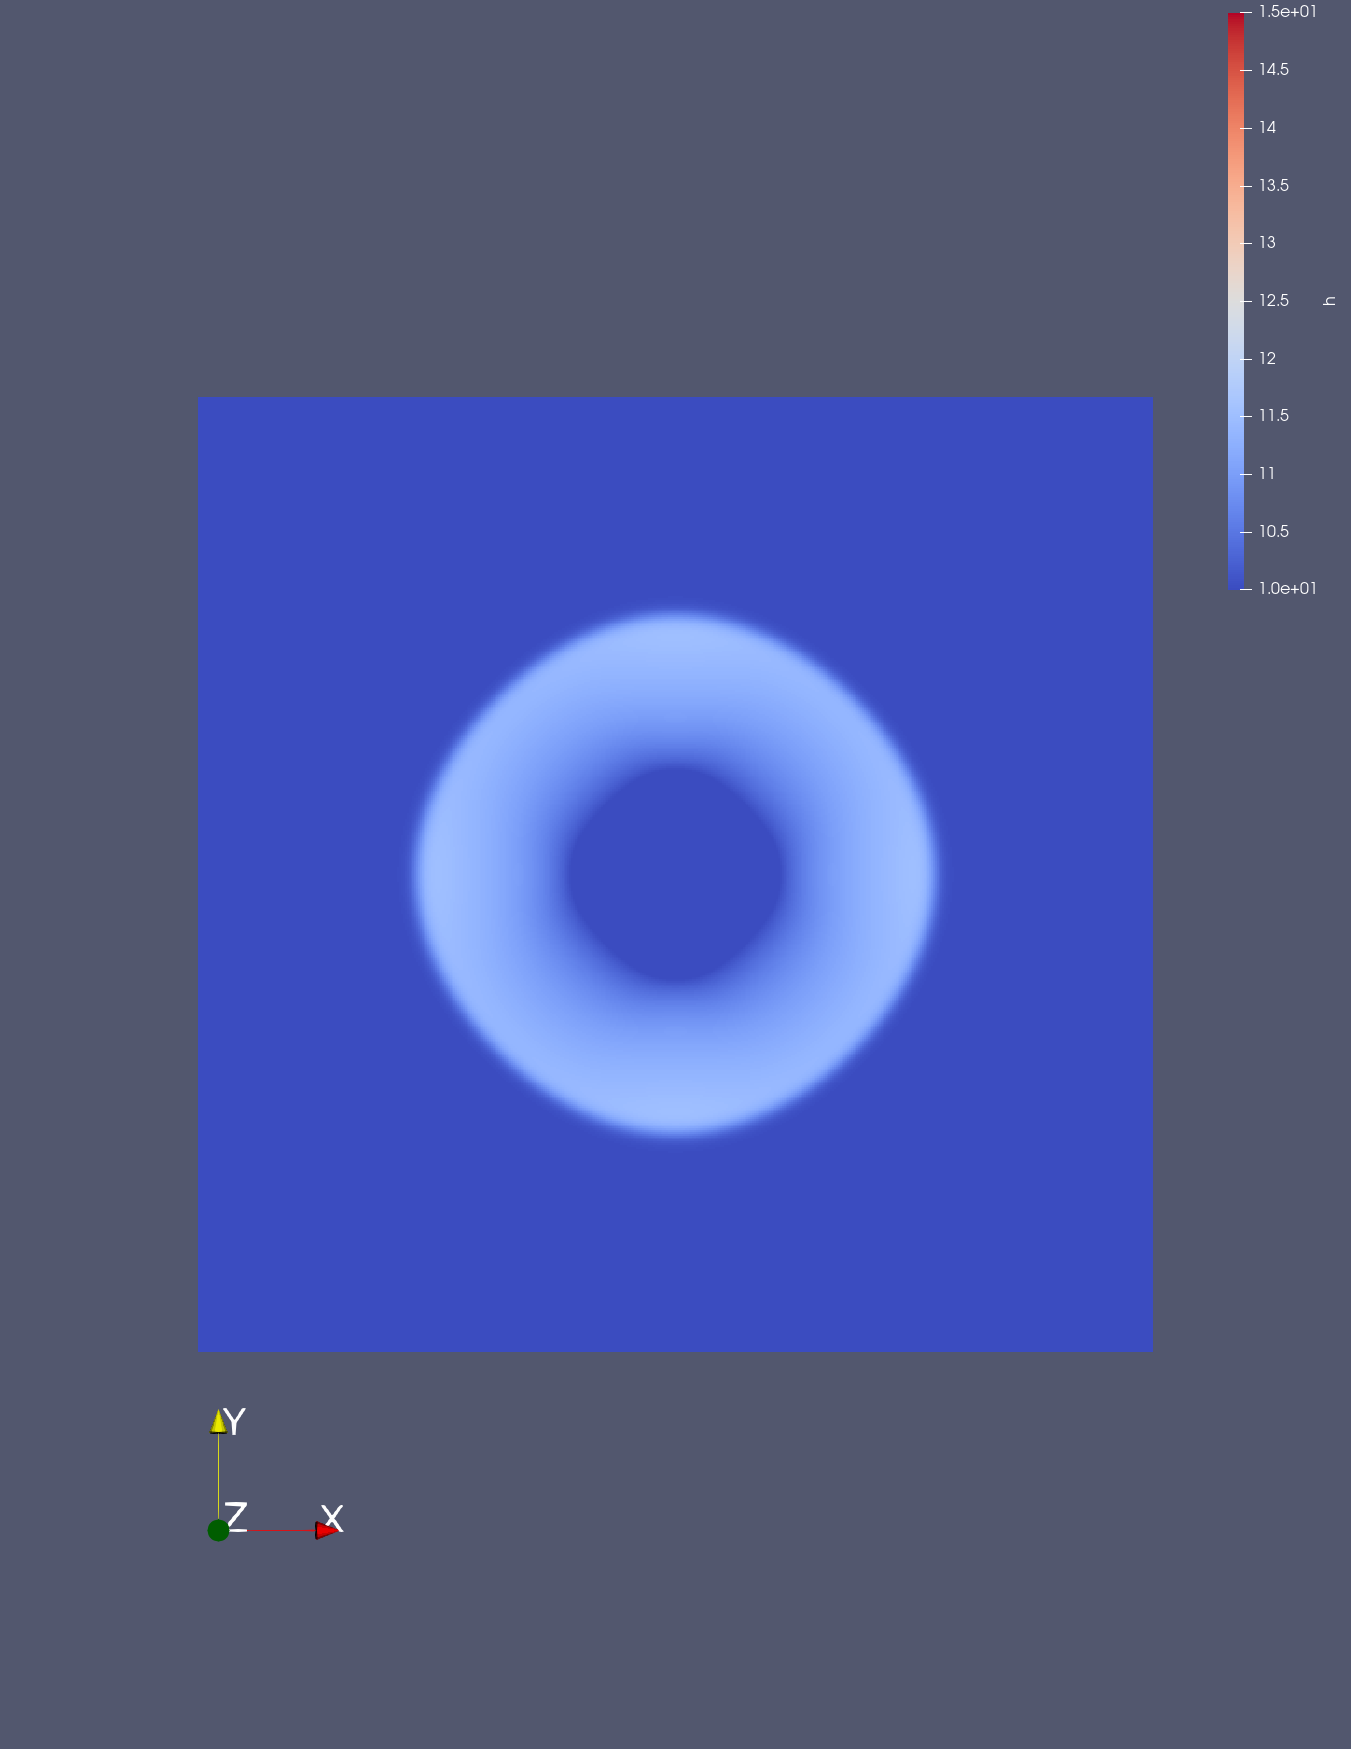
\includegraphics[width=\textwidth,keepaspectratio=true]{../figs/1_validation_cuda_original_1mpi.png}
        \caption{1 MPI (no CUDA)}
        \label{fig:1mpi}
    \end{subfigure}
%
    \begin{subfigure}{.3\textwidth}
    \centering
    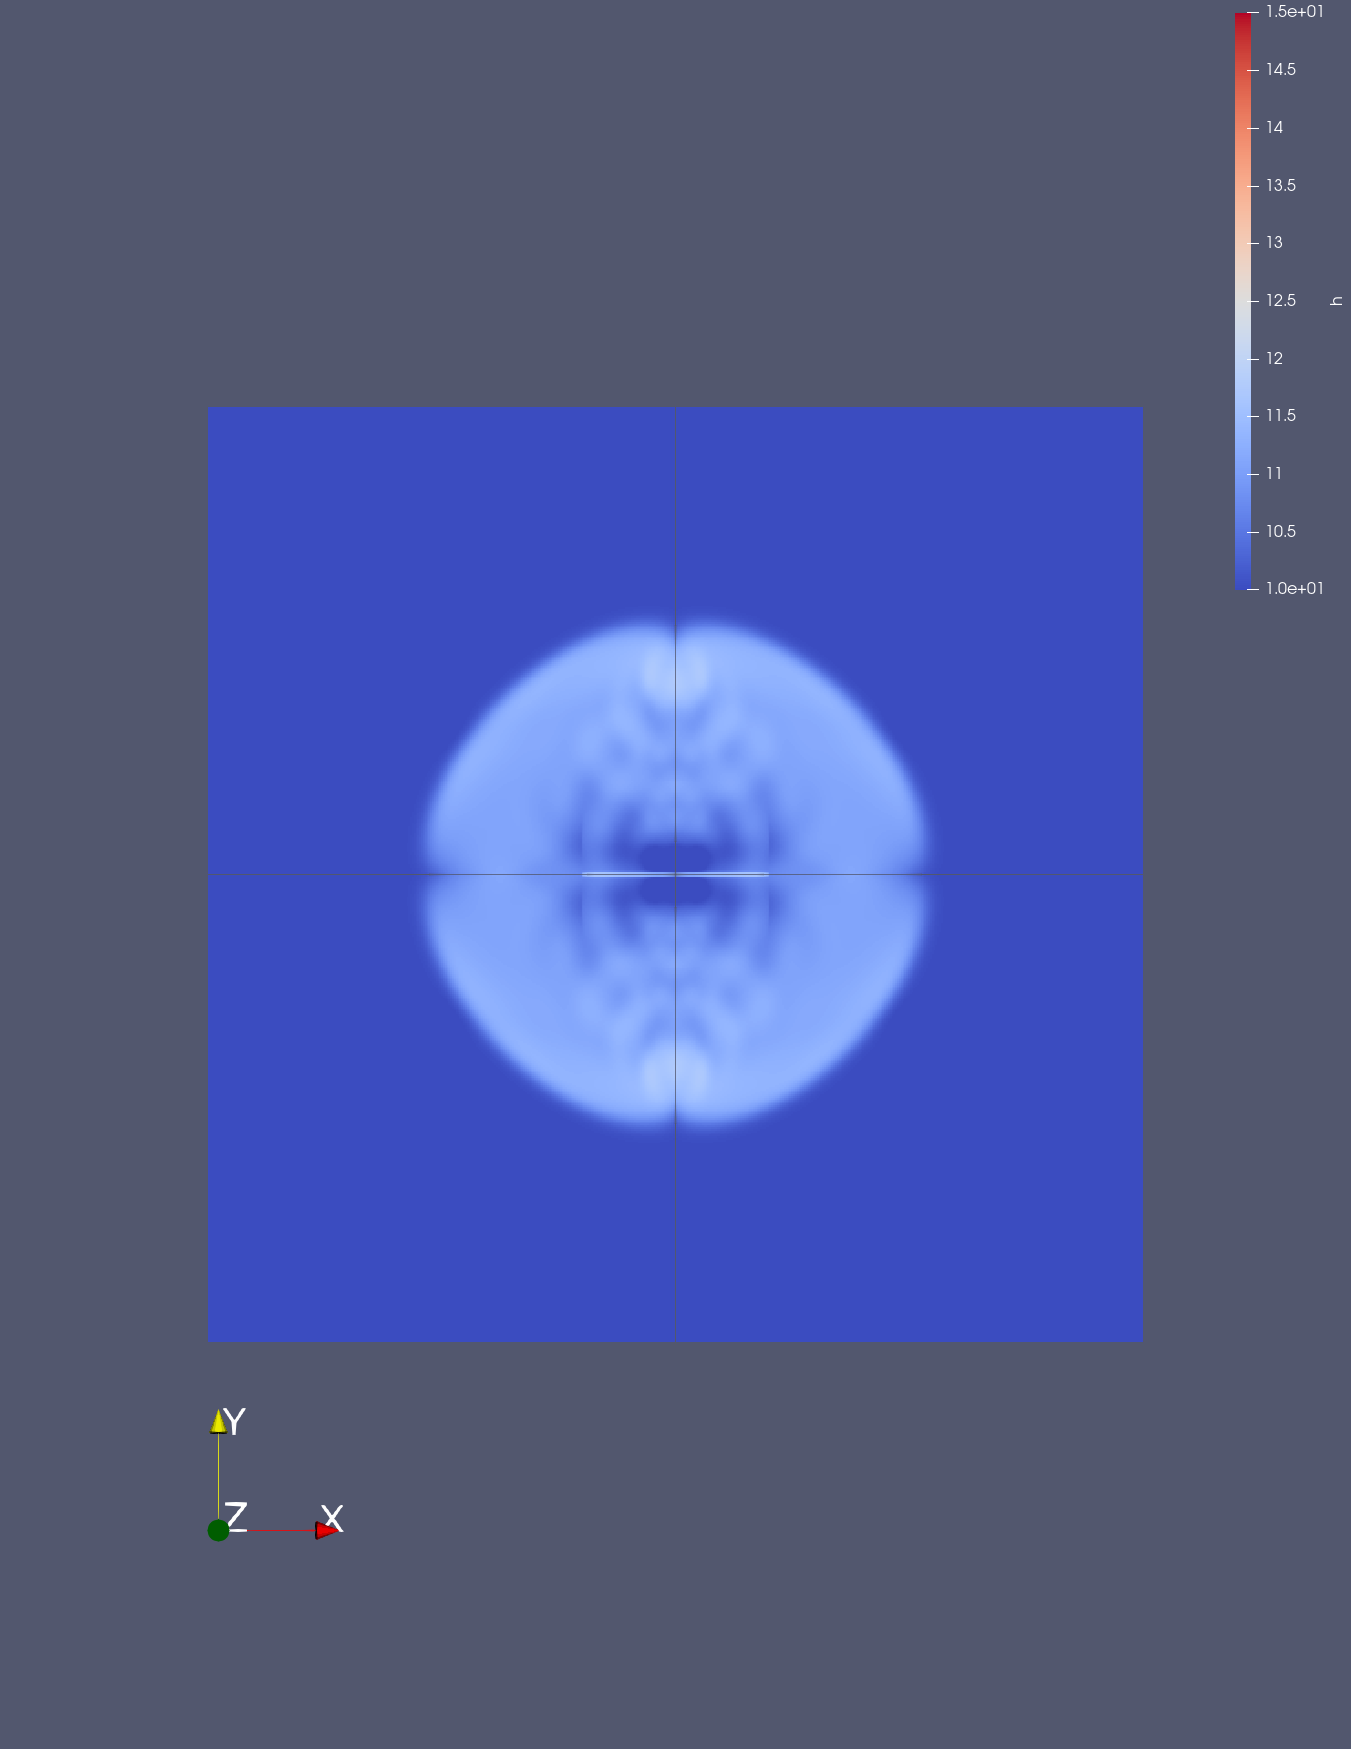
\includegraphics[width=\textwidth,keepaspectratio=true]{../figs/1_validation_cuda_original_4mpi.png}
    \caption{4 MPI-CUDA (before)}
    \label{fig:1mpi-cuda-original}
    \end{subfigure}
%
    \begin{subfigure}{.3\textwidth}
    \centering
    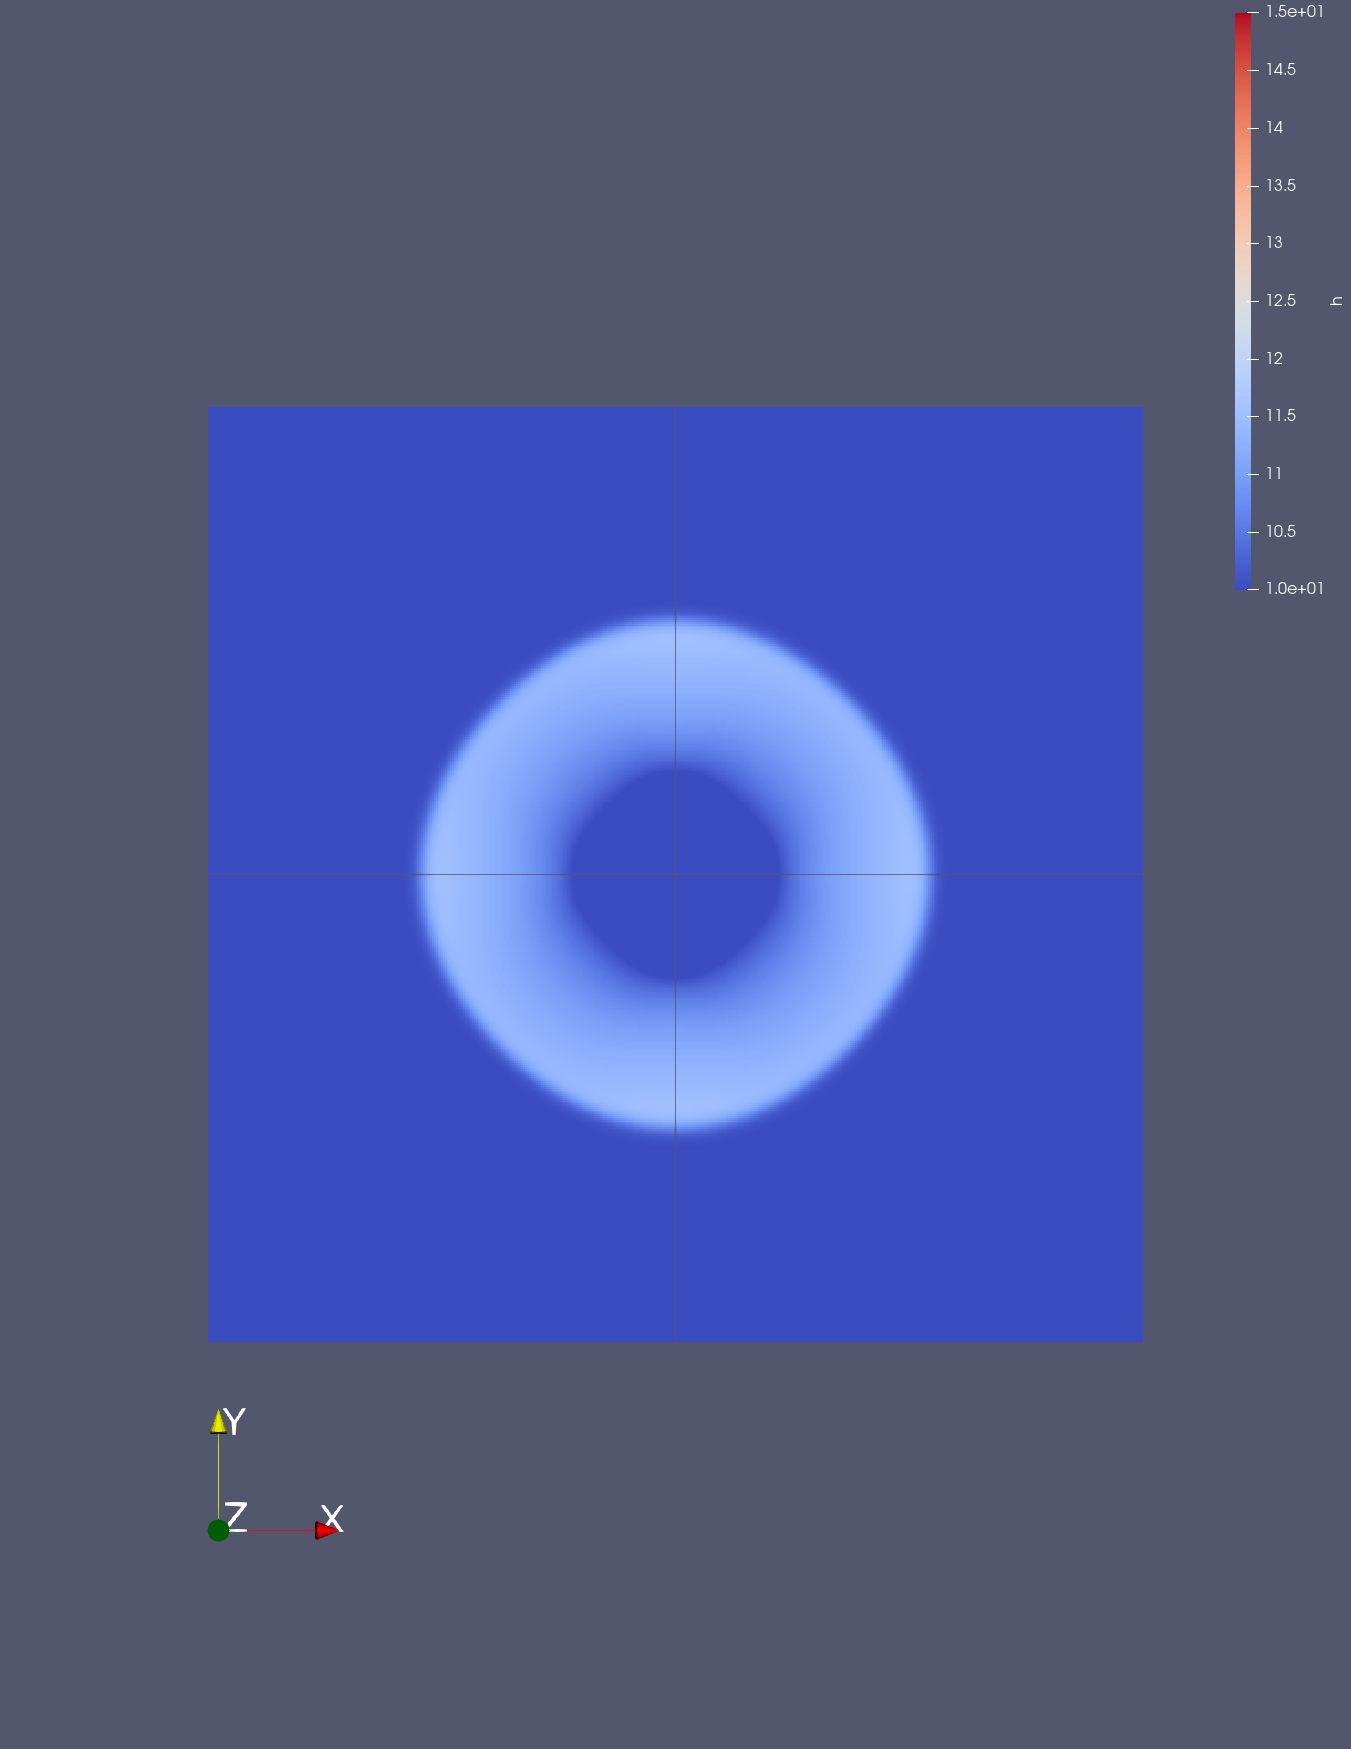
\includegraphics[width=\textwidth,keepaspectratio=true]{../figs/1_validation_cuda_fixed_4mpi.png}
    \caption{4 MPI-CUDA (after)}
    \label{fig:1mpi-cuda-fixed}
    \end{subfigure}
    \caption{Comparison of Visualisation of SWE CUDA before and after fixing bugs}
    \label{figs:validation_cuda}
\end{figure}

\begin{figure}[htpb]
  \centering
  \begin{subfigure}{.49\textwidth}
        \begin{tabular}{ |c|c|c|c|}
          \hline
                & 1 cuda      & 4 mpi  & 4 cuda \\
          \hline
          1 mpi & 0.02754     & 0.03729& 29929.4505 \\
          \hline
          1 cuda& 0.00000     & 0.06483& 29929.4468\\
          \hline
        \end{tabular}
    \caption{Before}
    \label{table:cuda_before}
  \end{subfigure}
%
    \begin{subfigure}{.49\textwidth}
    \centering
        \begin{tabular}{ |c|c|c|c|}
          \hline
                & 1 cuda      & 4 mpi  & 4 cuda \\
          \hline
          1 mpi & 0.02754     & 1.28397& 0.02754 \\
          \hline
          1 cuda& 0.00000     & 1.31151& 0.00000\\
          \hline
        \end{tabular}
    \caption{After}
    \label{table:cuda_after}
    \end{subfigure}

    \caption{Absolute differences of \textit{WaterHeight (h)} - Before and After fixing bugs}
    \label{table:cuda}
\end{figure}

\subsubsection{Validation of the CUDA-Aware MPI implementation}

%- Visualisation of output files: the same for normal MPI without CUDA and the CUDA-Aware MPI. (PUT 1 figures which has 3 subfigures for 1 mpi, 4 cuda, 4 cuda-aware) \\
We also did the same validation for our CUDA-Aware MPI version. The results are shown in the Figure~\ref{figs:validation_cuda_aware} and the Table~\ref{table:cuda_aware}. There is still a small error propagated from the \textit{1 mpi} - \textit{1 cuda} which is the same as in the previous session, thus can be neglected in this project. Our implementation, based on the original CUDA kernels, resulted exactly the same results as the CUDA versions. It means our implementation is correct and reliable. 
\begin{figure}[htpb]
    \centering
    \begin{subfigure}{.3\textwidth}
        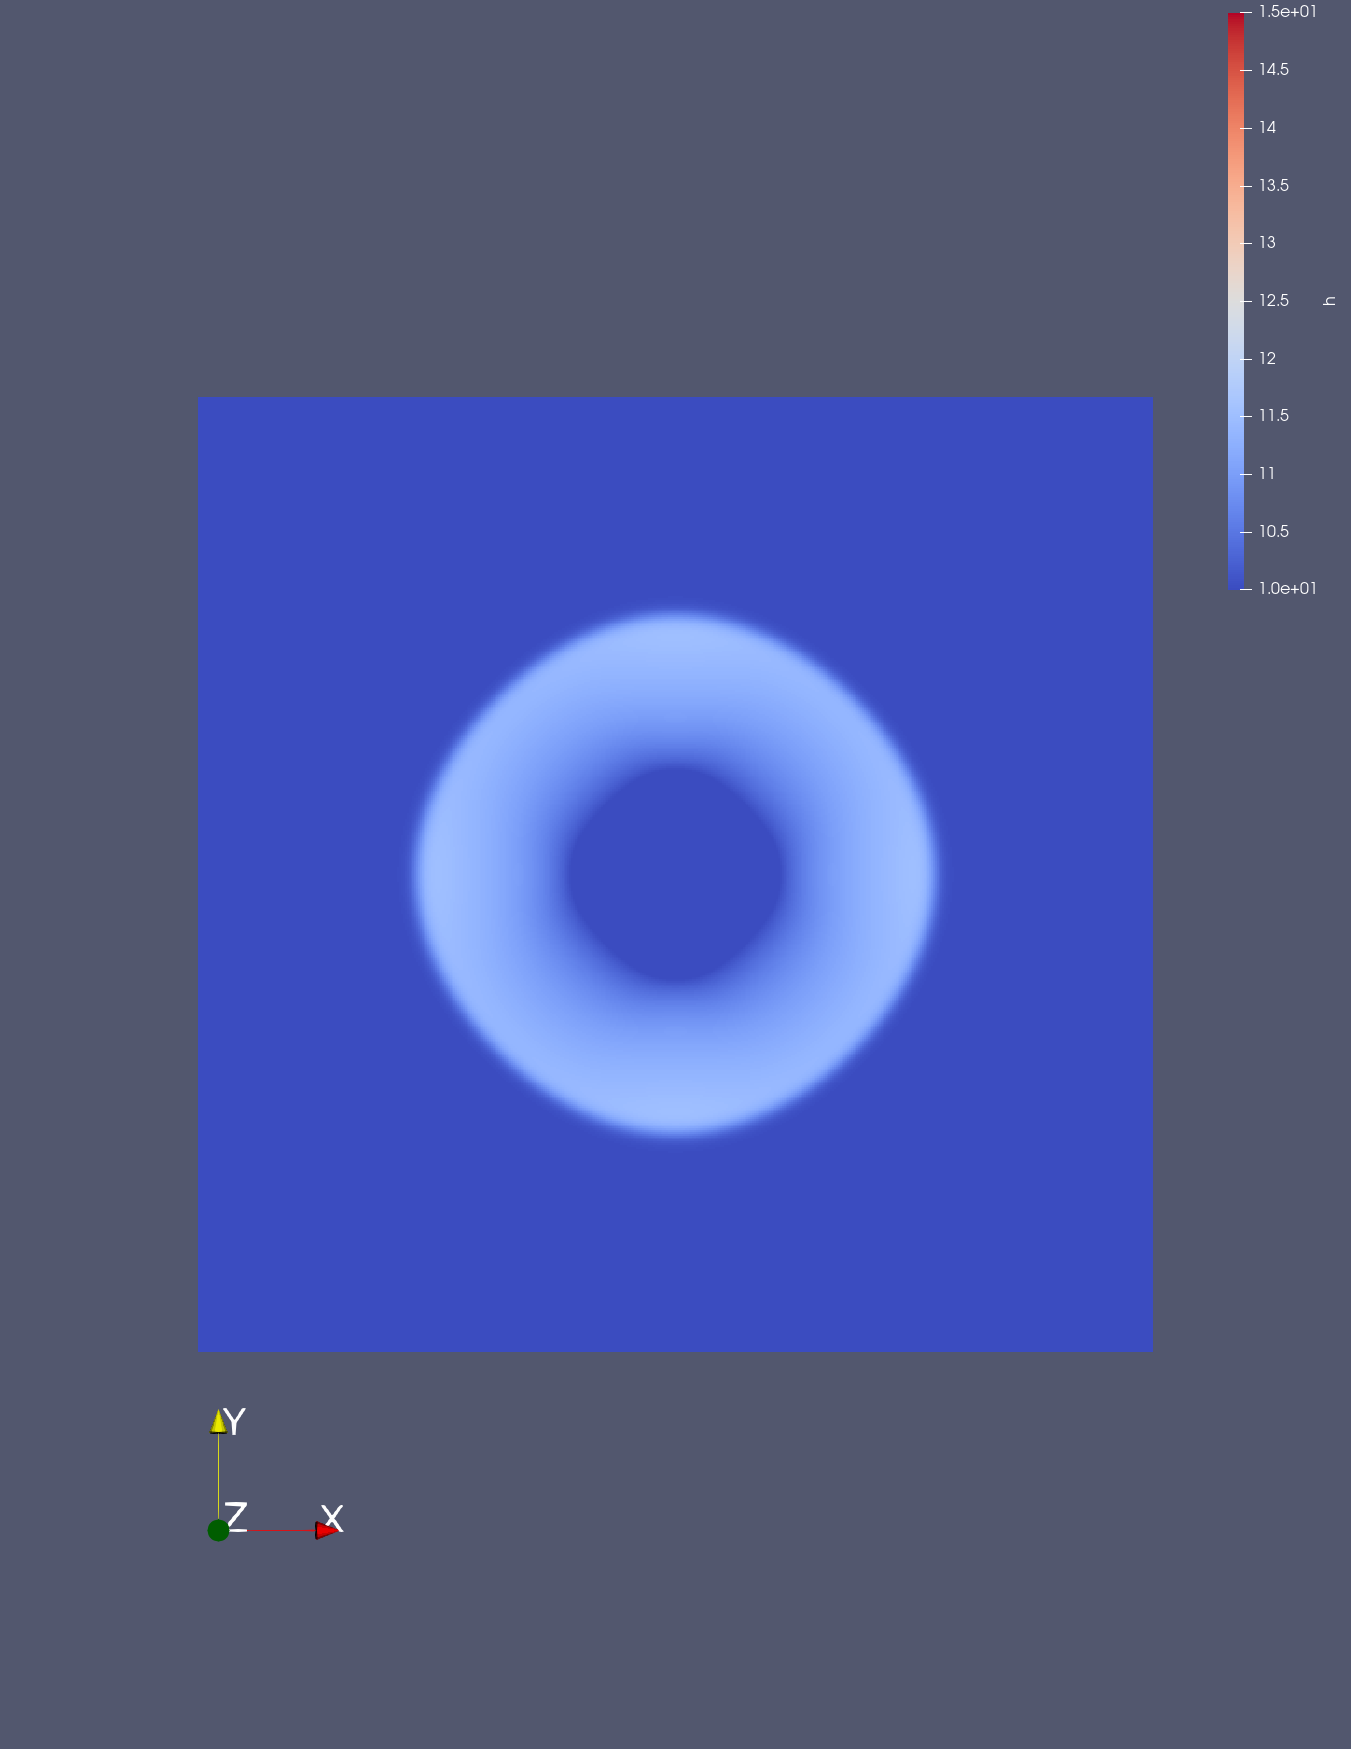
\includegraphics[width=\textwidth,keepaspectratio=true]{../figs/1_validation_cuda_original_1mpi.png}
        \caption{1 MPI (no CUDA)}
        \label{fig:1mpi_2nd}
    \end{subfigure}
%
    \begin{subfigure}{.3\textwidth}
    \centering
    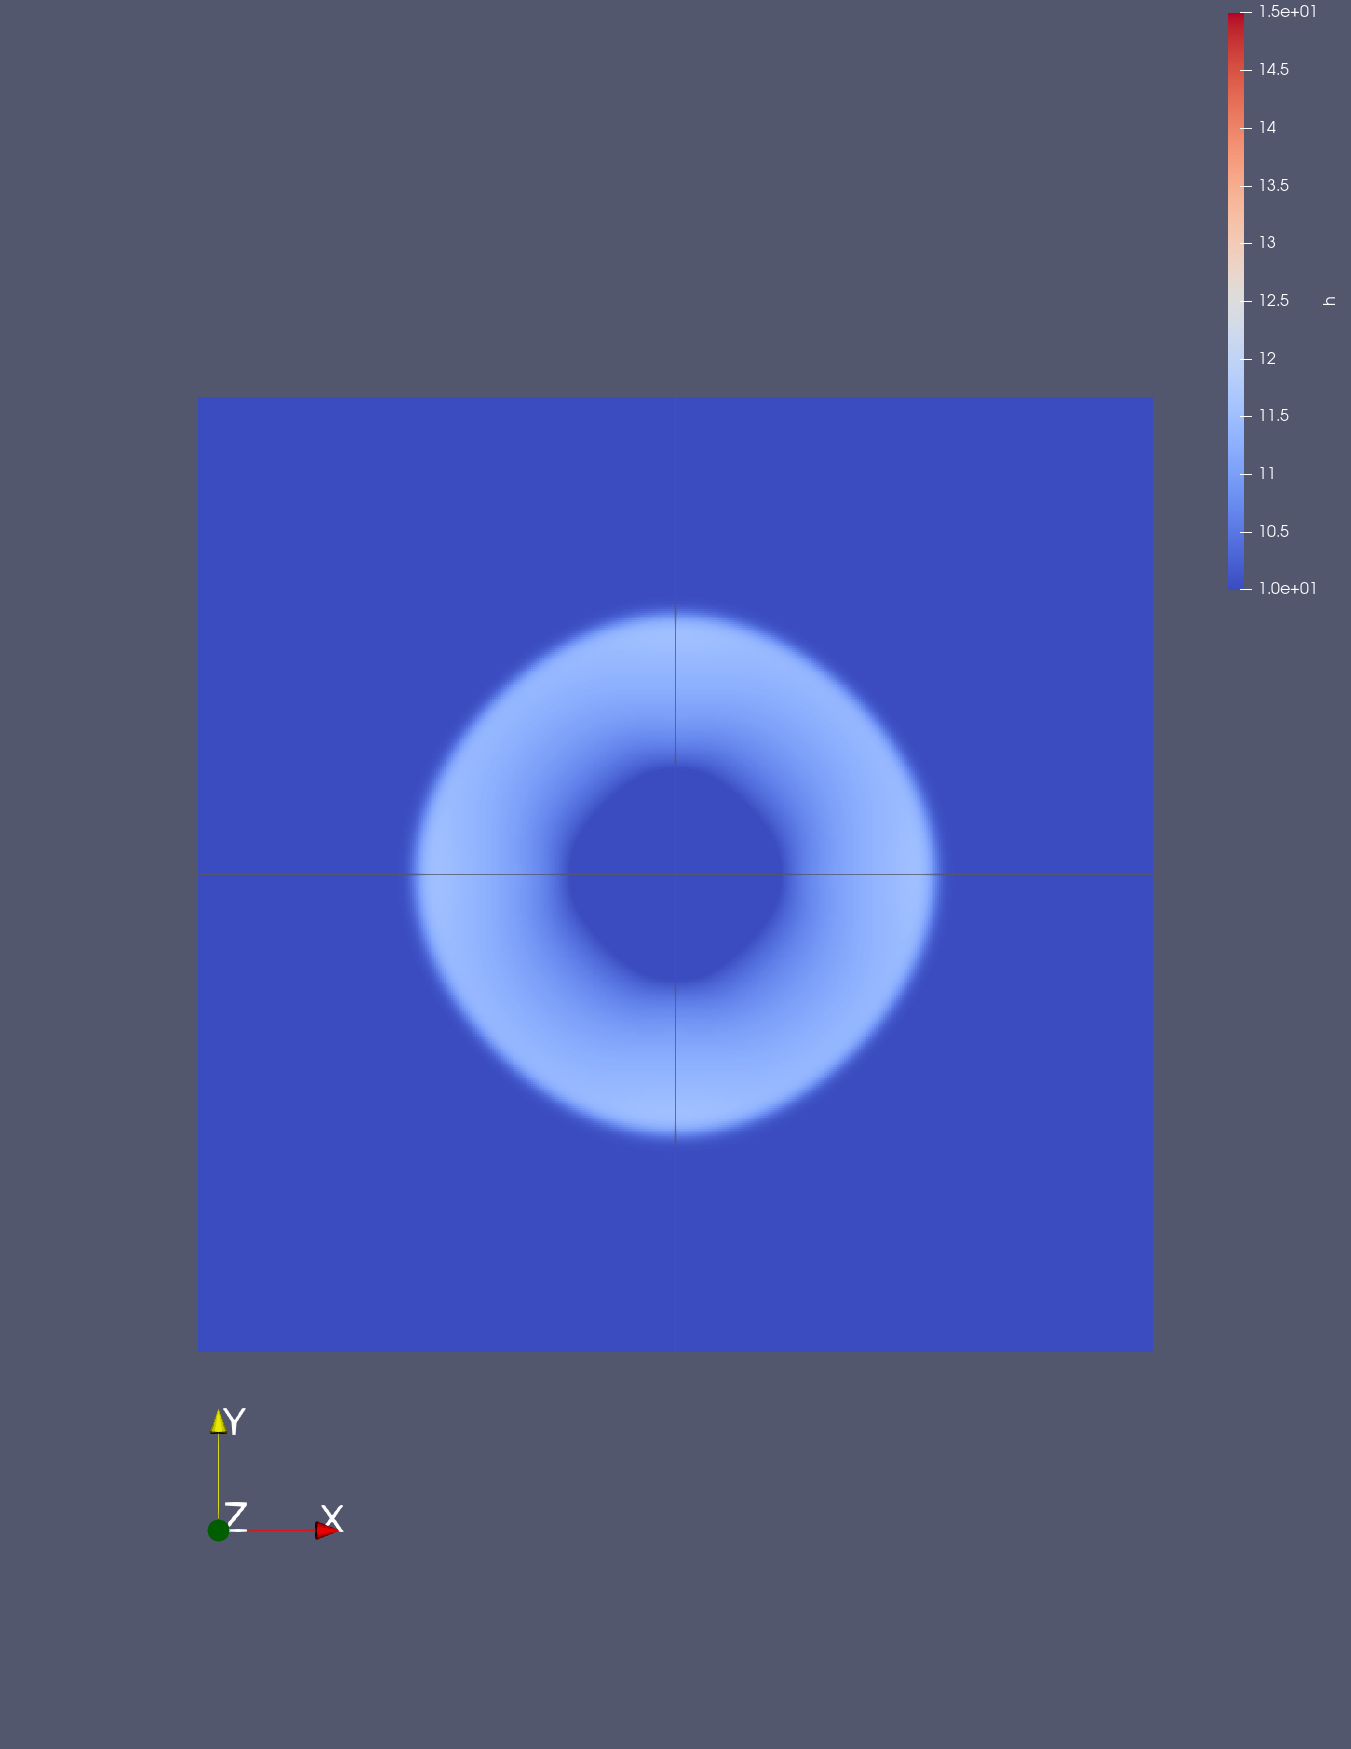
\includegraphics[width=\textwidth,keepaspectratio=true]{../figs/1_validation_cuda_aware_4mpi.png}
    \caption{4 CUDA-Aware-MPI)}
    \label{fig:4mpi-cuda-aware}
    \end{subfigure}
    \caption{Comparison of Visualisation of SWE: pure-MPI vs CUDA-Aware-MPI}
    \label{figs:validation_cuda_aware}
\end{figure}

\begin{table}[h!]
  \centering
\begin{tabular}{ |c|c|c|}
  \hline
        & 1 cuda-aware& 4 cuda-aware \\
  \hline
  1 mpi & 0.02754     & 0.02754 \\
  \hline
  1 cuda& 0.00000     &  0.00000 \\
  \hline
  4 cuda& 0.00000     & 0.00000 \\
  \hline
\end{tabular}
\caption{Absolute differences of \textit{WaterHeight (h)} - Between purely MPI, CUDA, and CUDA-Aware MPI Implementation}
\label{table:cuda_aware}
\end{table}
%- Show that our run envolved all 4 GPUs (take a screenshot of nvidia-smi).\\
%- Automated Regression Test (table show errors). \\
\subsection{Initial result}
%- Run 1 2 4 GPUs, we got a plot. Strong scaling test. 1 figures compare strong scaling of cuda vs cuda-aware. 1 figures for parallel efficient of cuda-aware. \\
We tested our implementation with different grid sizes and number of GPUs, the performance of our CUDA-Aware-MPI, in comparision to the original CUDA implementation, are shown in Figure~\ref{figs:Compare1} and Figure~\ref{figs:Compare2}. 
%- 1 figures for computational time. \\
\begin{figure}[htpb!]
	\centering
	\begin{subfigure}{.48\textwidth}
		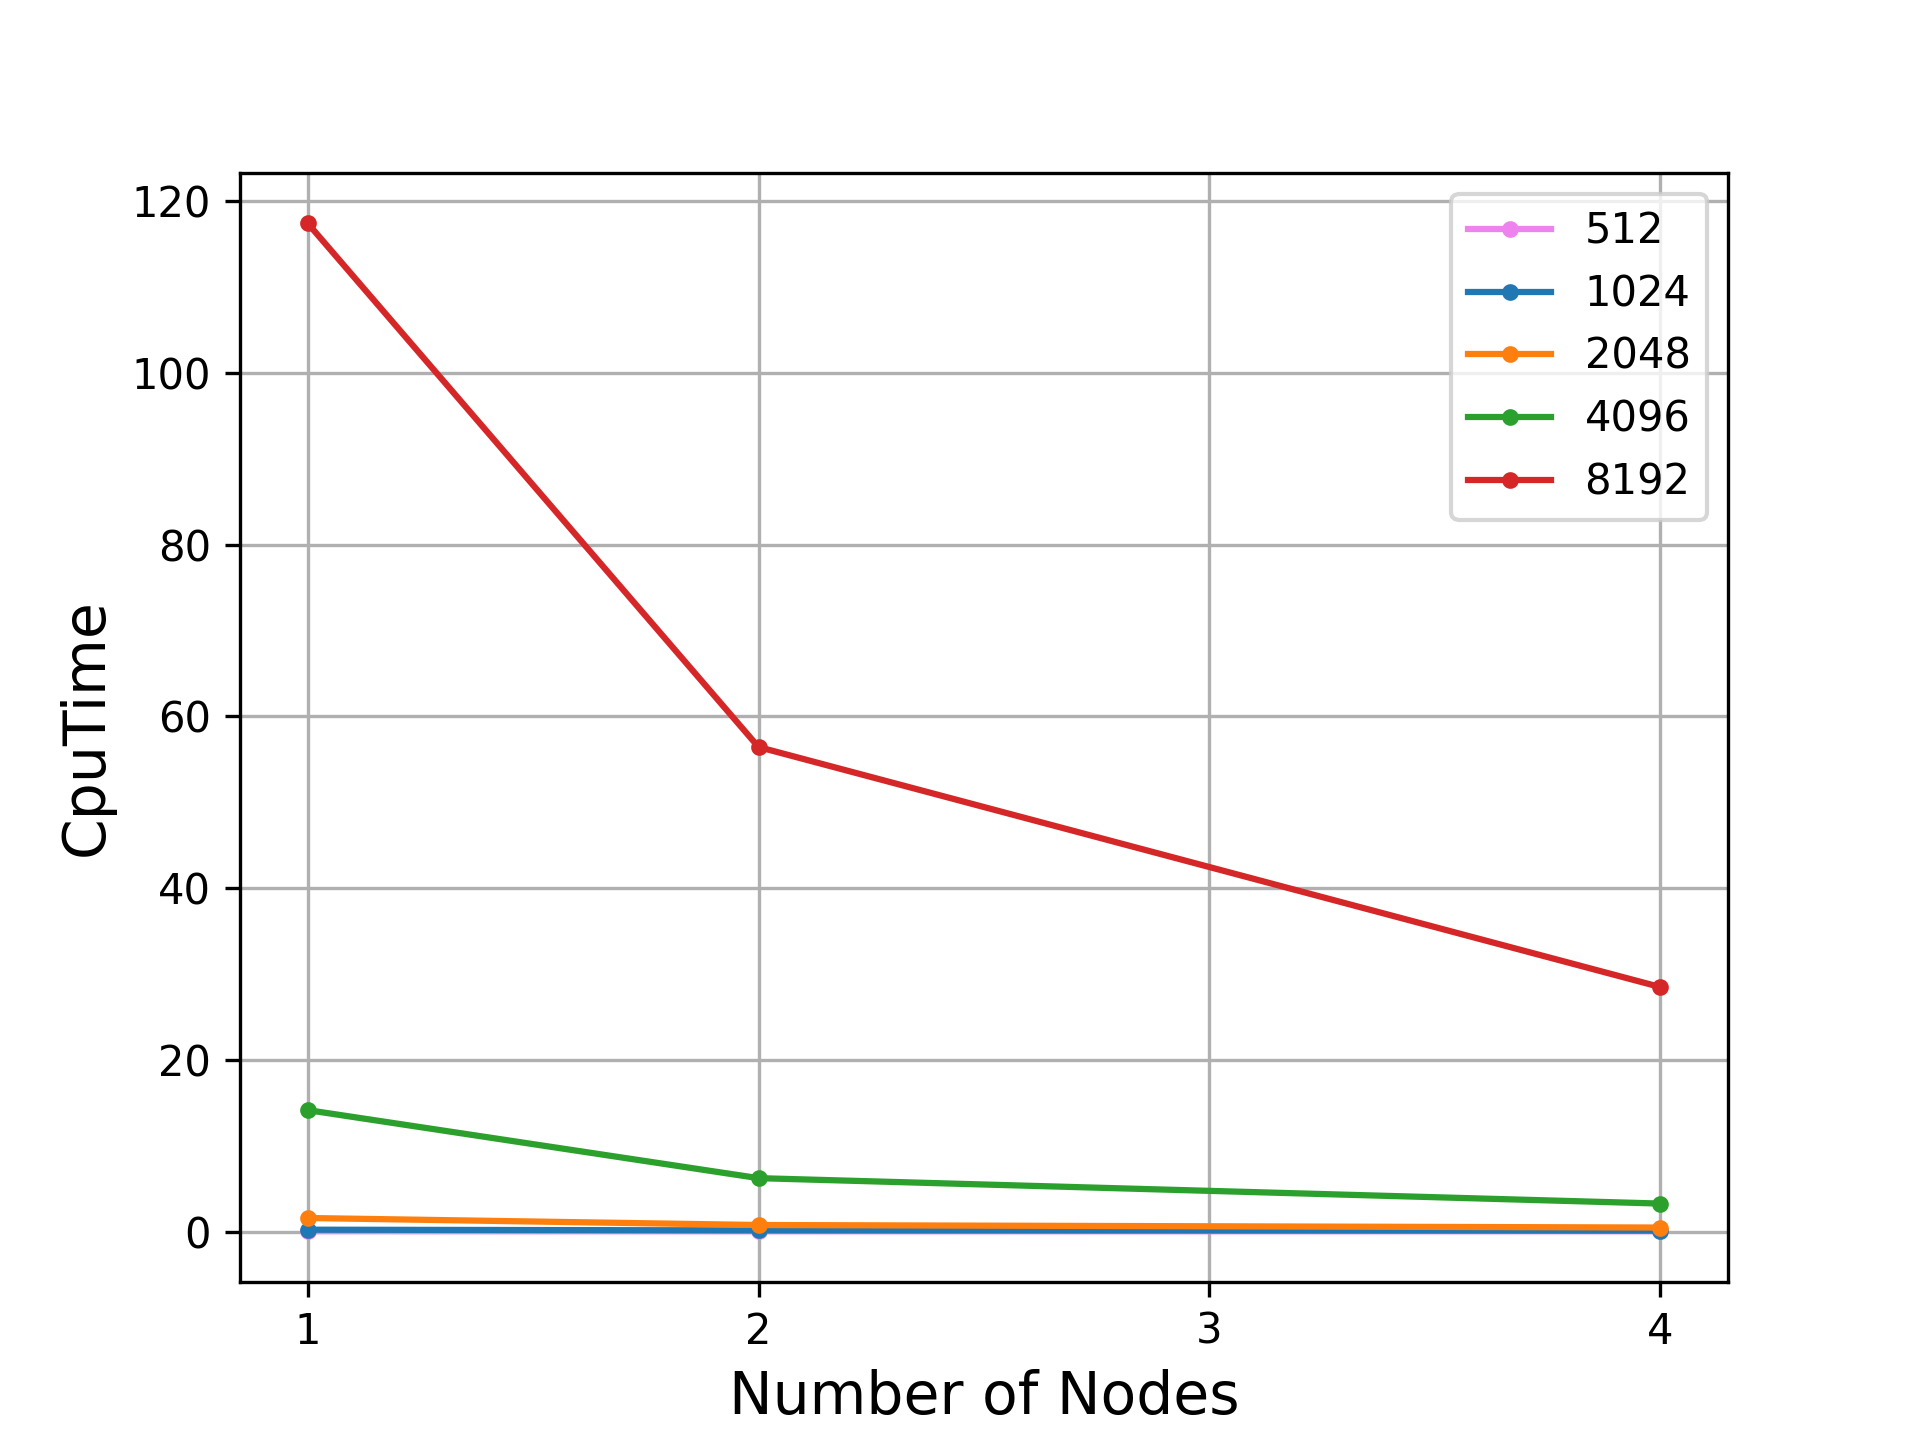
\includegraphics[width=\textwidth,keepaspectratio=true]{../figs/strongscalingCPU_CUDA.png}
		\caption{normal CUDA+MPI}
		\label{fig:StrongCpuCUDA}
	\end{subfigure}
	%
	\begin{subfigure}{.48\textwidth}
		\centering
		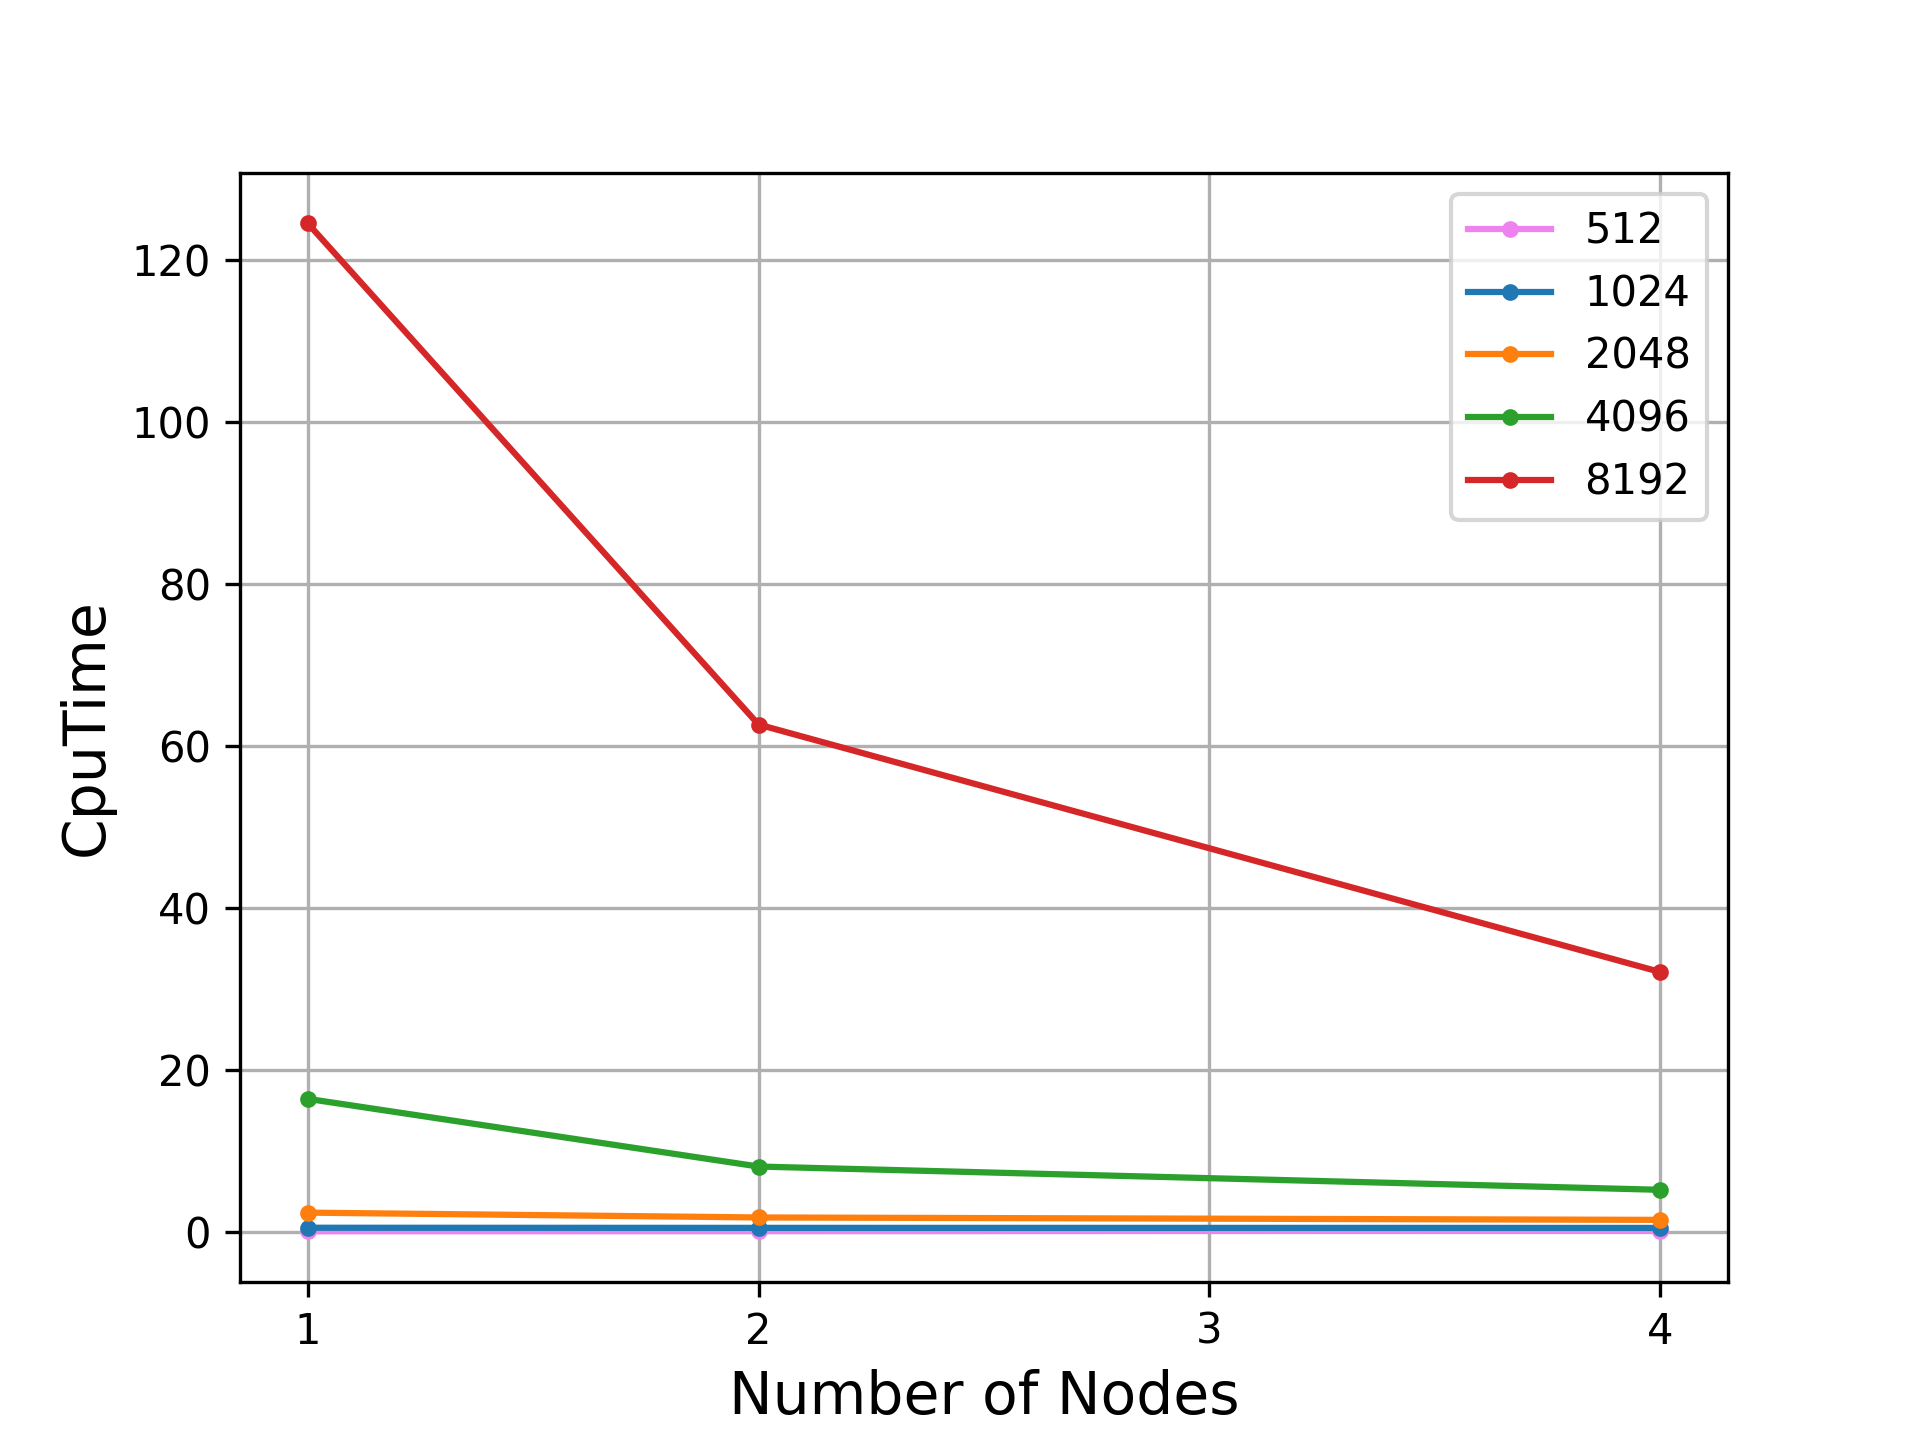
\includegraphics[width=\textwidth,keepaspectratio=true]{../figs/strongscalingCPU.png}
		\caption{CUDA-Aware-MPI}
		\label{fig:StrongCpu}
	\end{subfigure}
	
	\caption{Computation-Time (or CPU-Time) comparison of the two implementations with different grid sizes (Strong-scaling)}
	\label{figs:Compare1}
\end{figure}

In Figure~\ref{figs:Compare1}, we see that there is no big difference between normal CUDA+MPI and CUDA-Aware-MPI with respect to the CPU time, just the time spent by CUDA-Aware-MPI is a bit more. Although they both use the same GPU resources for computing, CUDA-Aware-MPI requires Hardware/Software to migrate pages automatically while this is done manuelly in normal CUDA. So a bit more overhead should be acceptable. 

In Figure~\ref{figs:Compare2}, the CPU+Communication time of normal CUDA+MPI stays almost the same as CPU time, which means the communication overhead is low. However, we observe a huge jump in \ref{fig:StrongCOMM} compared to \ref{fig:StrongCpu} when it comes to 4 Nodes. Let's discuss about this in more detail. 
\begin{figure}[htpb]
	\centering
	\begin{subfigure}{.49\textwidth}
		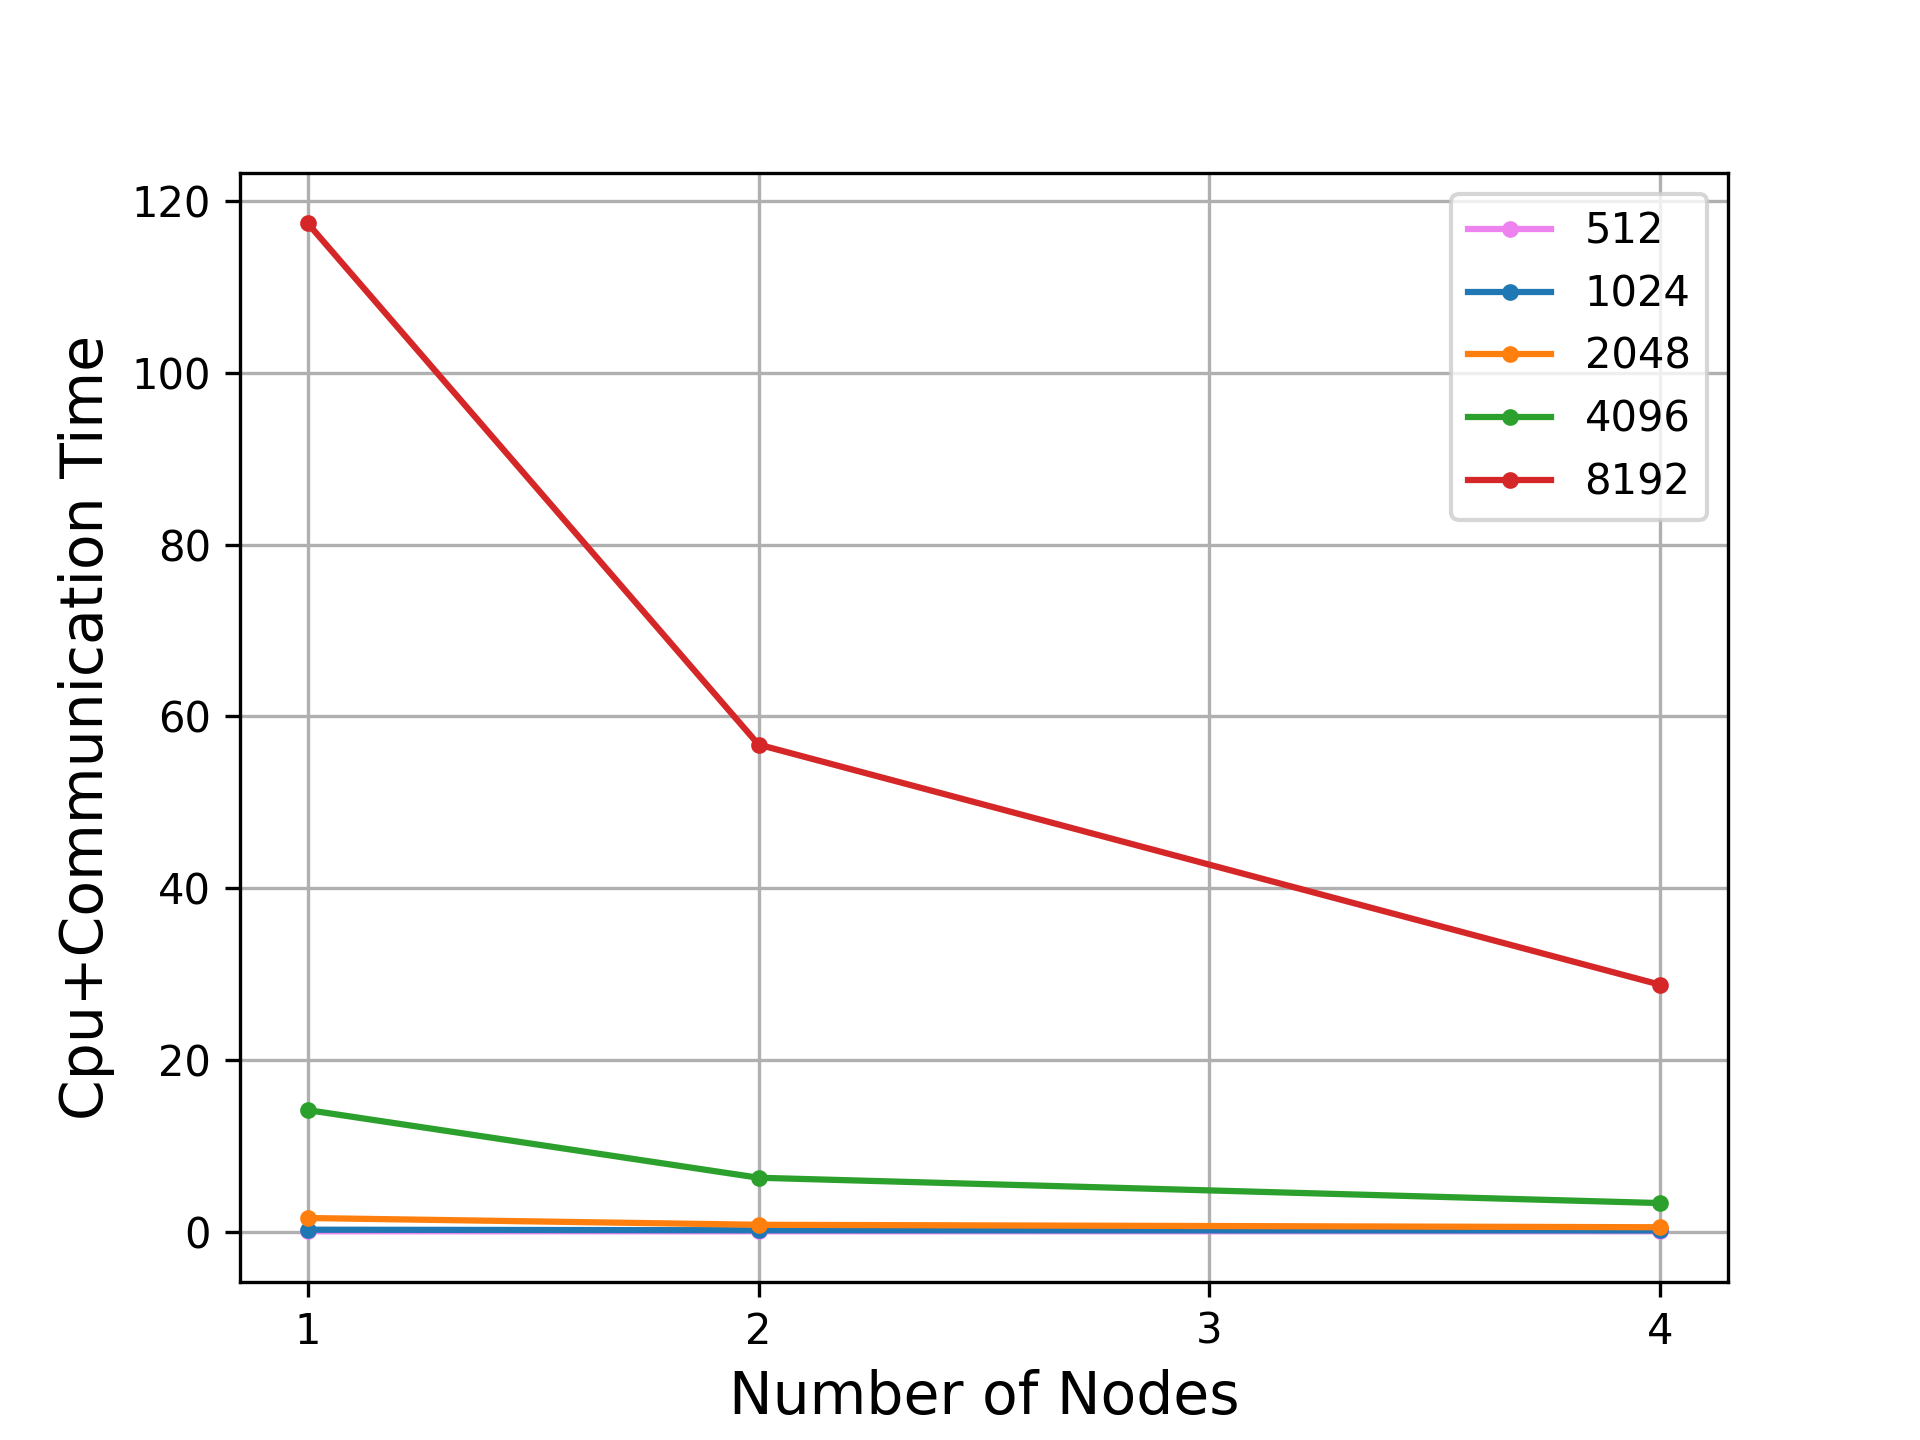
\includegraphics[width=\textwidth,keepaspectratio=true]{../figs/strongscalingCOMM_CUDA.png}
		\caption{normal CUDA+MPI}
		\label{fig:StrongCOMMCUDA}
	\end{subfigure}
	%
	\begin{subfigure}{.49\textwidth}
		\centering
		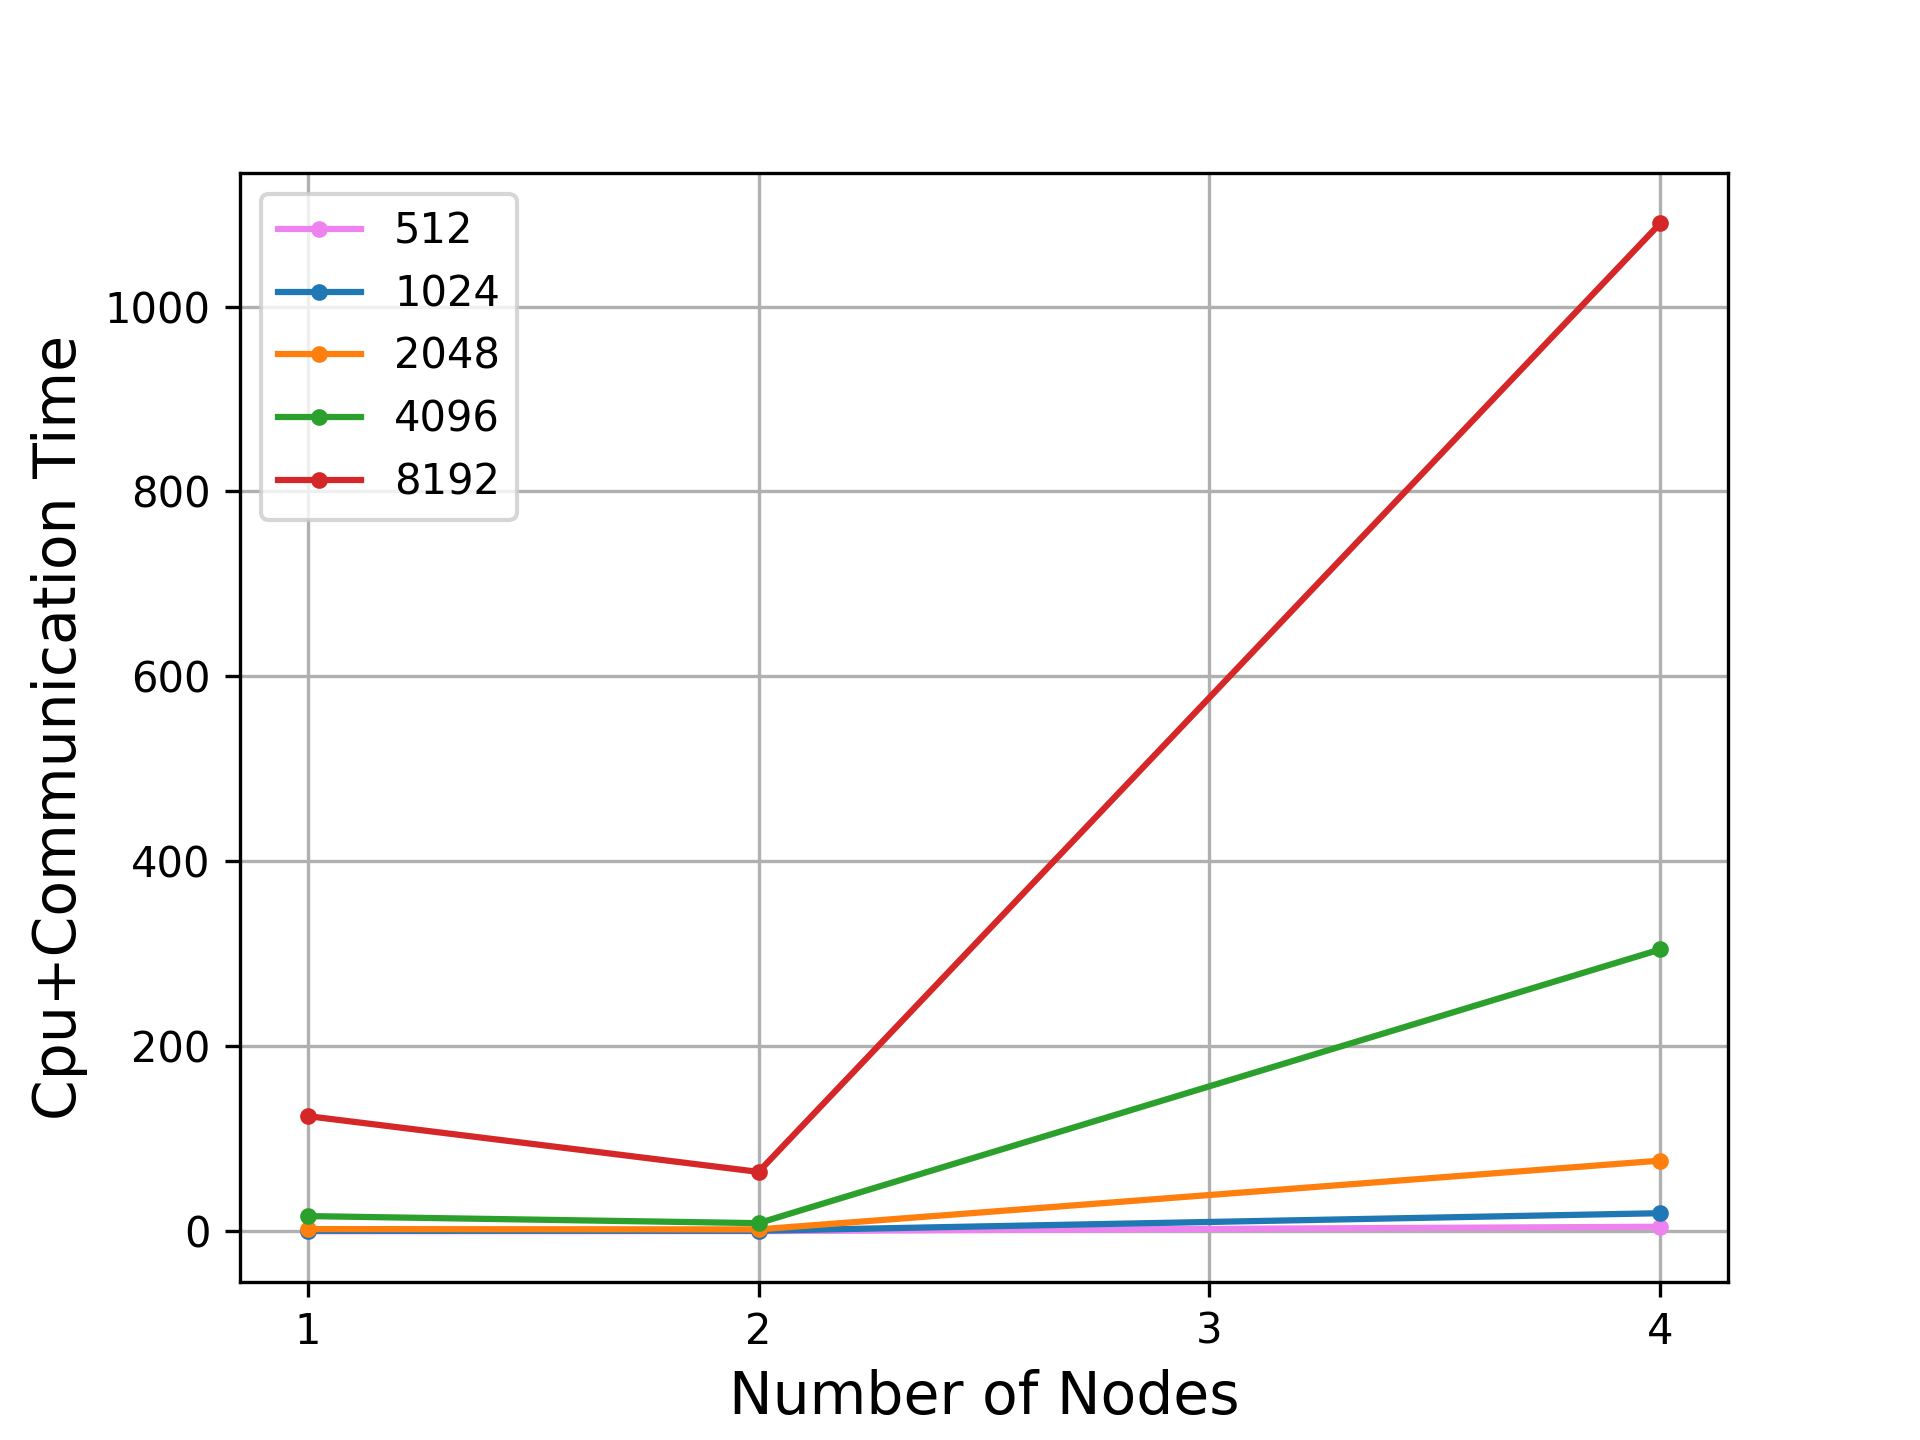
\includegraphics[width=\textwidth,keepaspectratio=true]{../figs/strongscalingCOMM.png}
		\caption{CUDA-Aware-MPI}
		\label{fig:StrongCOMM}
	\end{subfigure}
	\caption{TOTAL-Time comparison of the two implementations with different grid sizes (Strong-scaling)}
	\label{figs:Compare2}
\end{figure}
 
We checked the hardware specification again and find out that our GPUs model is the NVIDIA GeForce RTX™ 3080 which does not have NVLINK \cite{gpudirect, rtx3080}. Therefore, the channel for data movement between GPUs will be most likely through PCIe, which has way lower bandwidth than NVLINK. The system also does not support either GPUDirect RMDA or GPUDirect P2P. When two GPUs need to communicate with each other, without GPU Direct, the communication always need to go through Host (CPUs), thus the data need to be migrated to host before MPI communications. Thus, it is unlikely that we can have CUDA-Aware MPI perform better than the tradition CUDA implemetation, with the given hardware system. 

%\begin{figure}[htpb]
%    \centering
%    \begin{subfigure}{.4\textwidth}
%        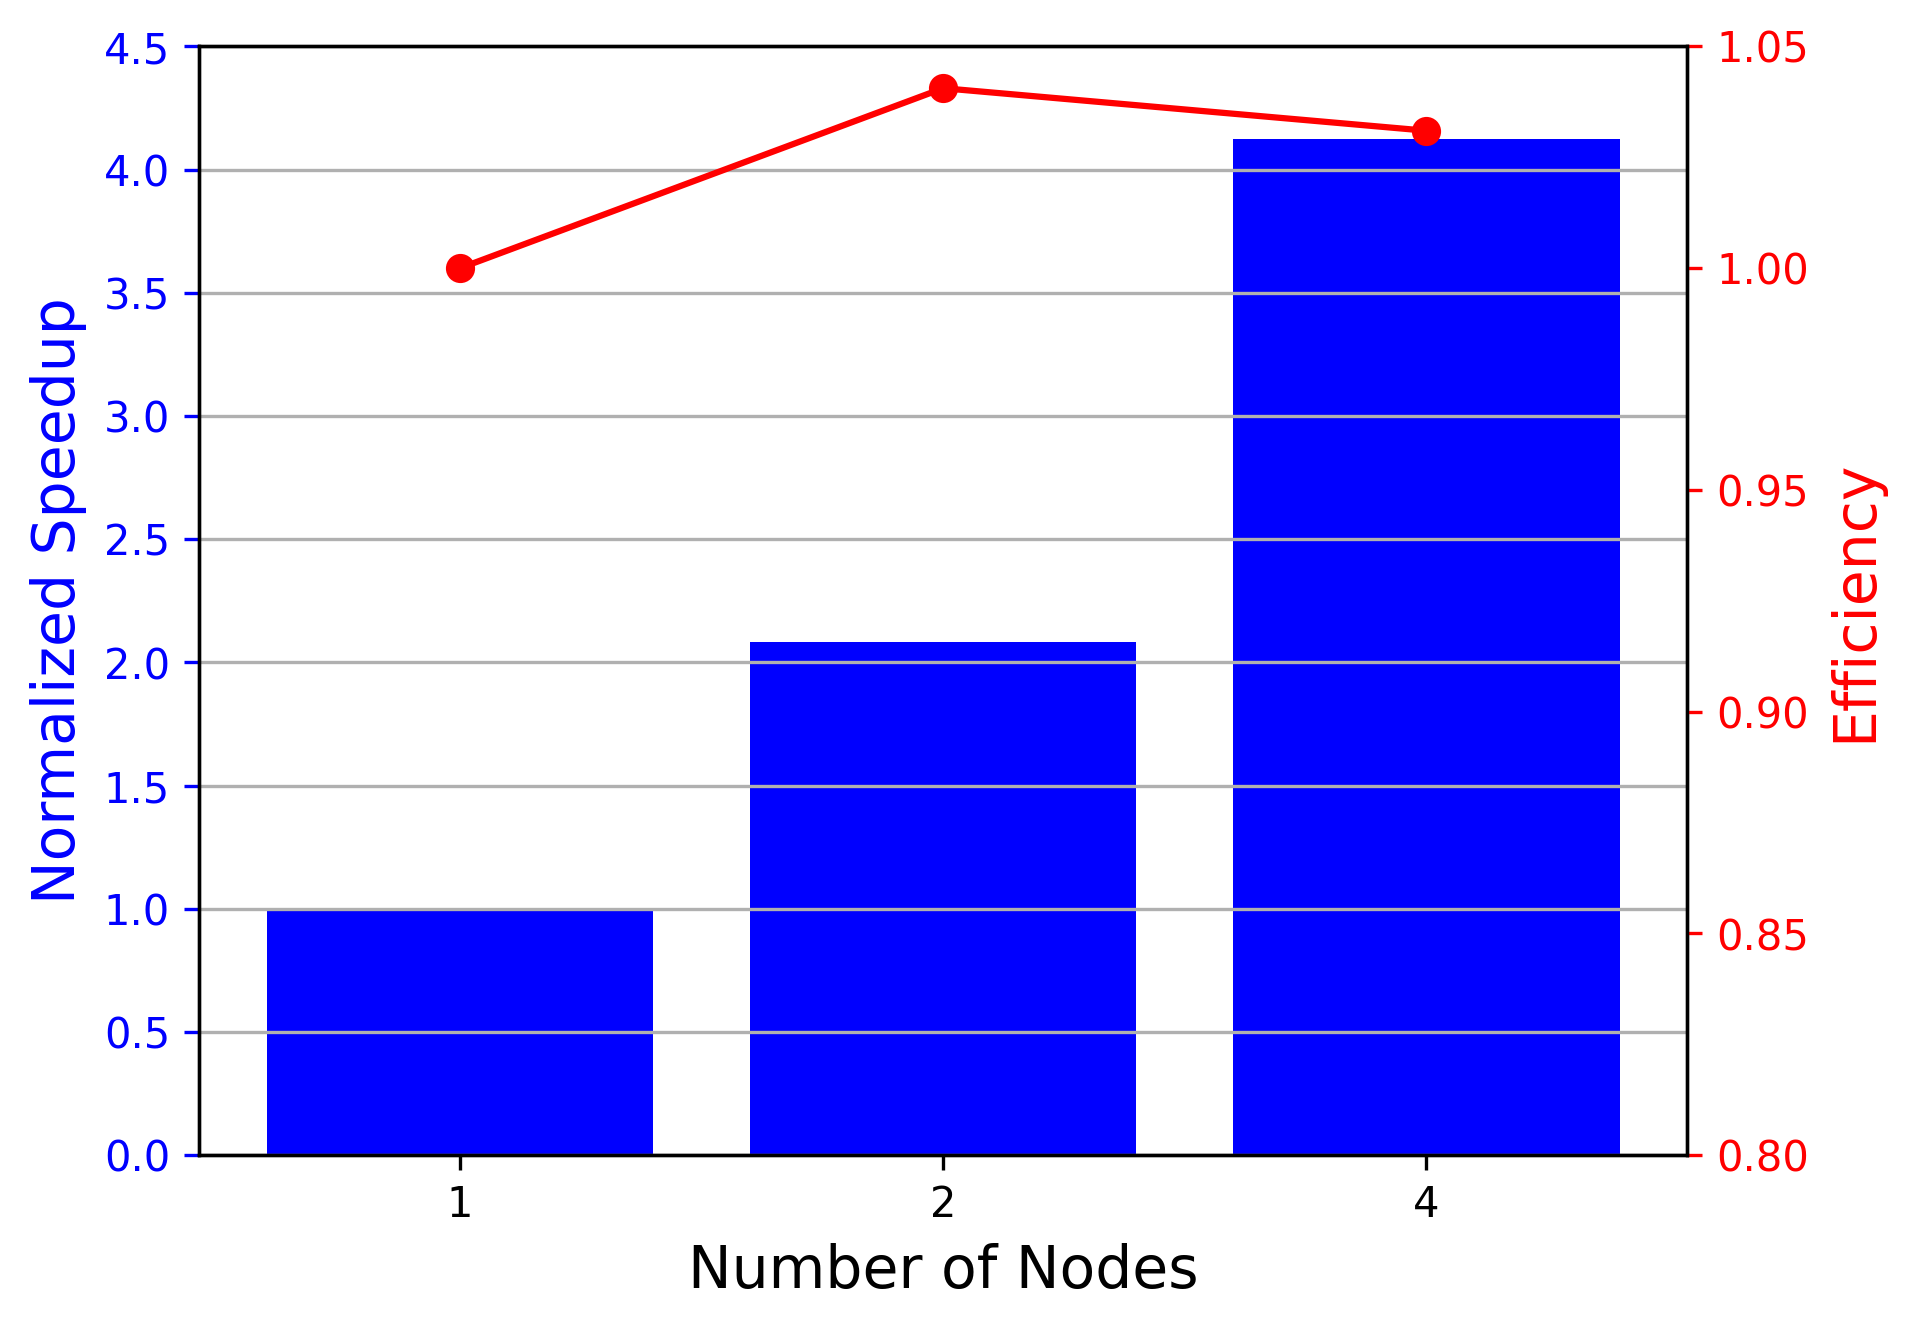
\includegraphics[width=\textwidth,keepaspectratio=true]{../figs/SpeedUp_Eff_CUDA.png}
%        \caption{normal CUDA+MPI}
%		\label{fig:SpeedEffCpuCUDA}
%    \end{subfigure}
%%
%    \begin{subfigure}{.4\textwidth}
%    \centering
%    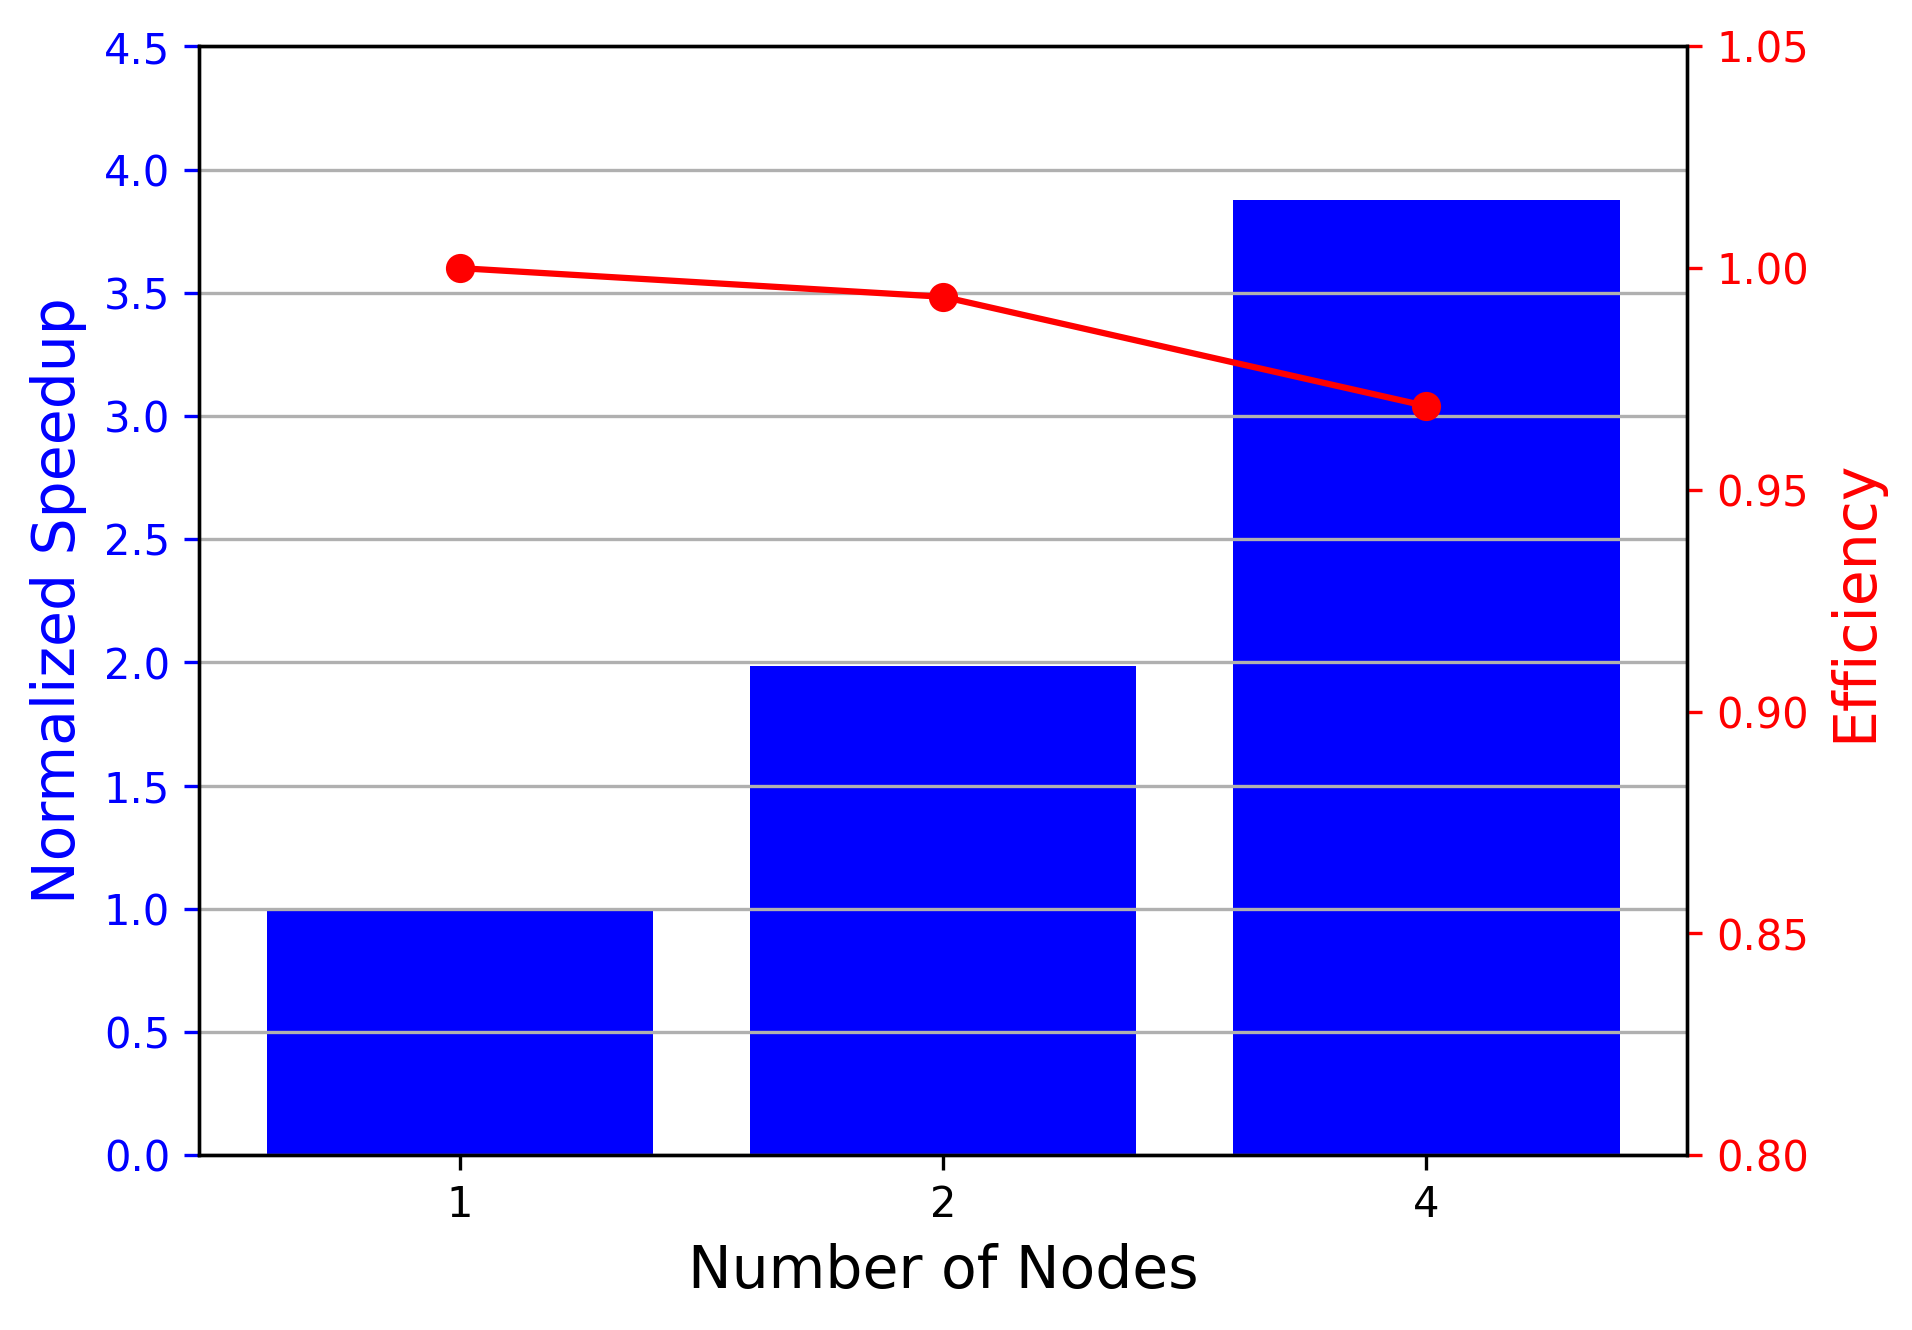
\includegraphics[width=\textwidth,keepaspectratio=true]{../figs/SpeedUp_Eff.png}
%    \caption{CUDA-Aware-MPI}
%	\label{fig:SpeedEffCpu}
%    \end{subfigure}
%    \caption{Comparison of SpeedUp and Efficiency using CPU Time As Metric with x, y = 8192 : normal CUDA+MPI vs CUDA-Aware-MPI}
%    \label{figs:Compare3}
%\end{figure}

%\begin{figure}[htpb]
%    \centering
%    \begin{subfigure}{.4\textwidth}
%        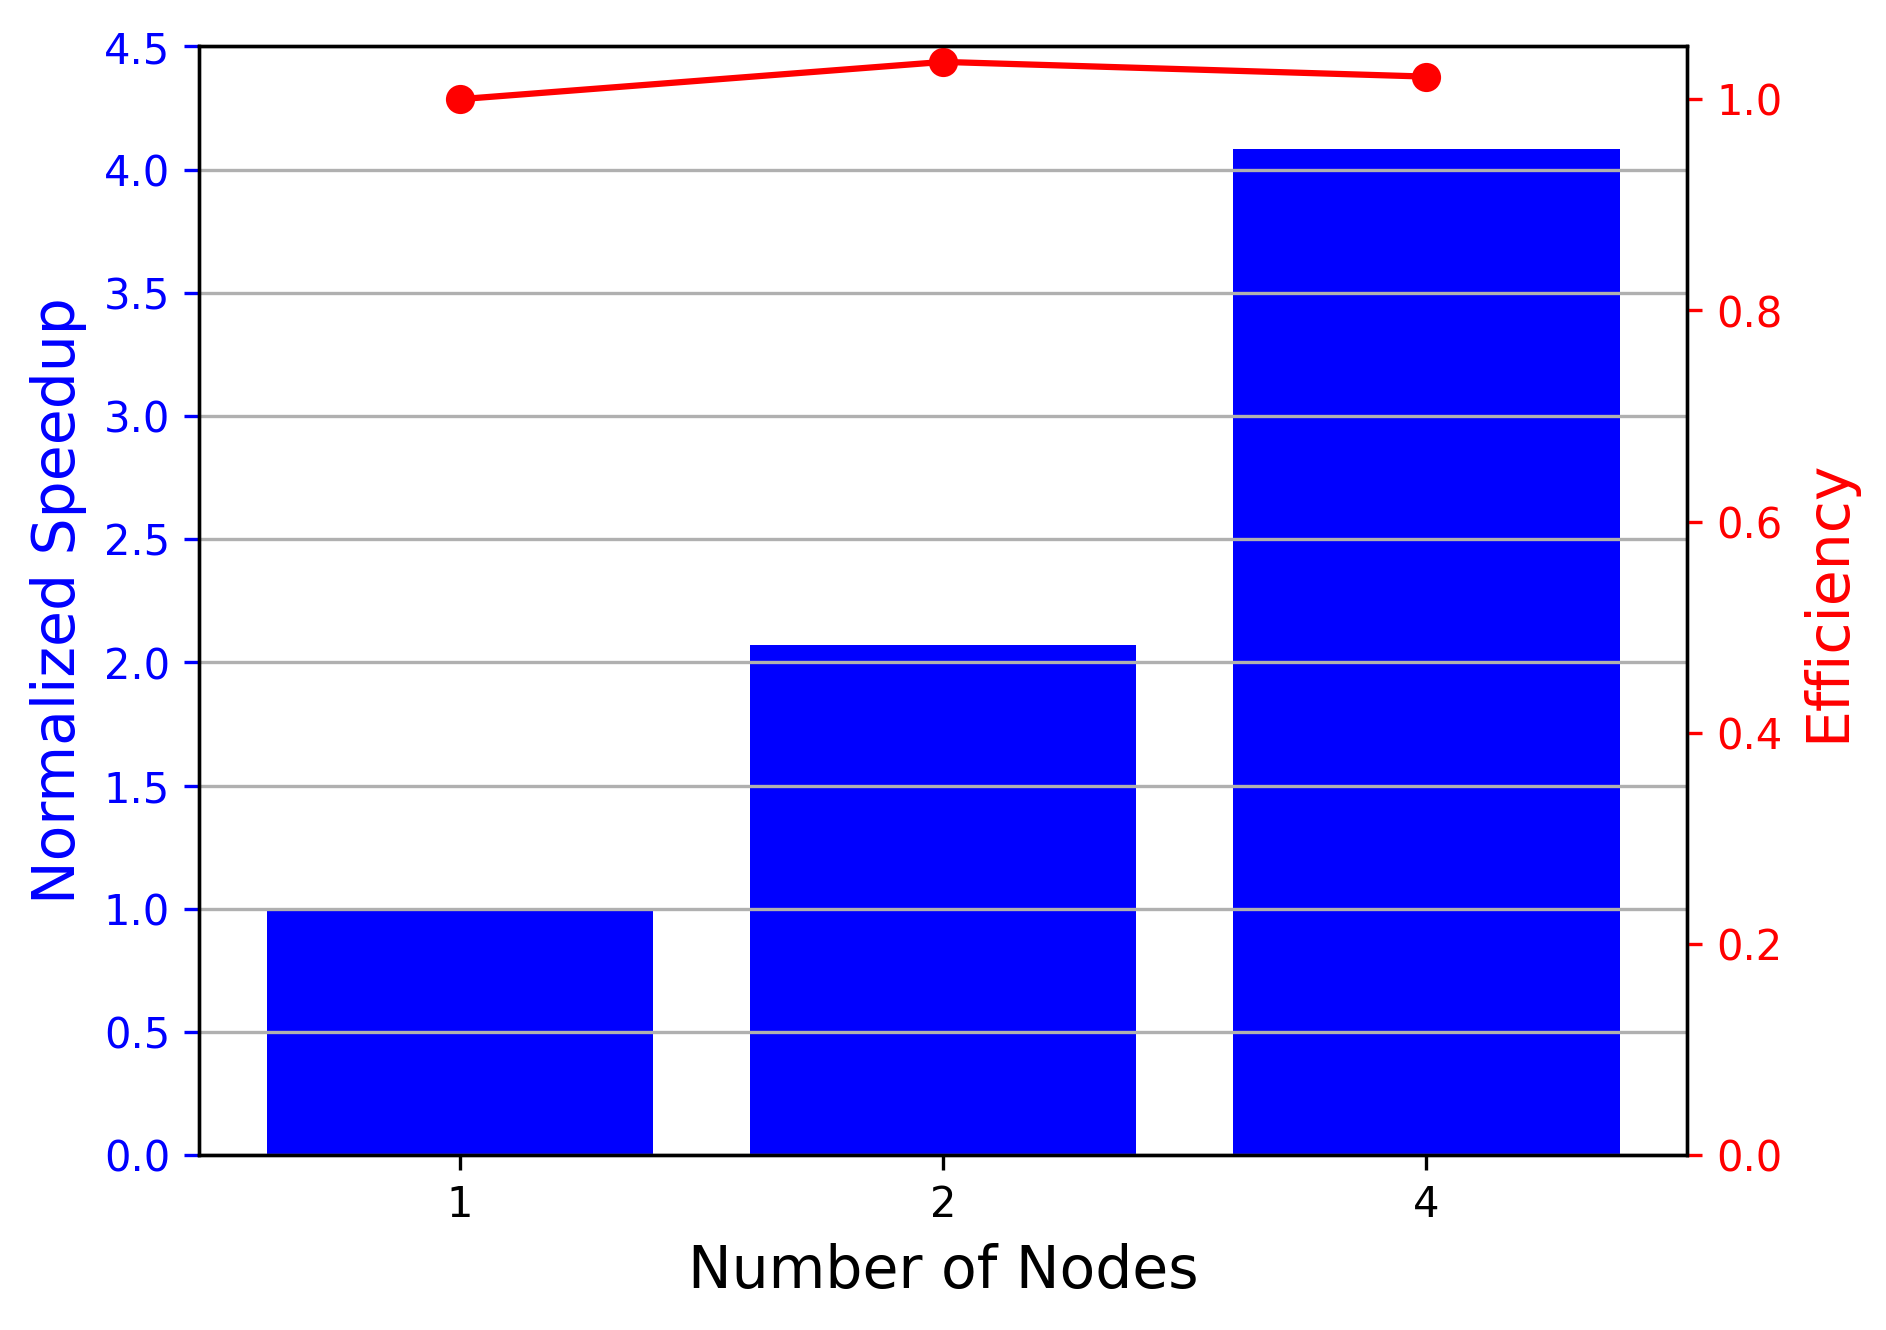
\includegraphics[width=\textwidth,keepaspectratio=true]{../figs/SpeedUp_Eff_COMM_CUDA.png}
%        \caption{normal CUDA+MPI}
%		\label{fig:SpeedEffCpuCUDA}
%    \end{subfigure}
%%
%    \begin{subfigure}{.4\textwidth}
%    \centering
%    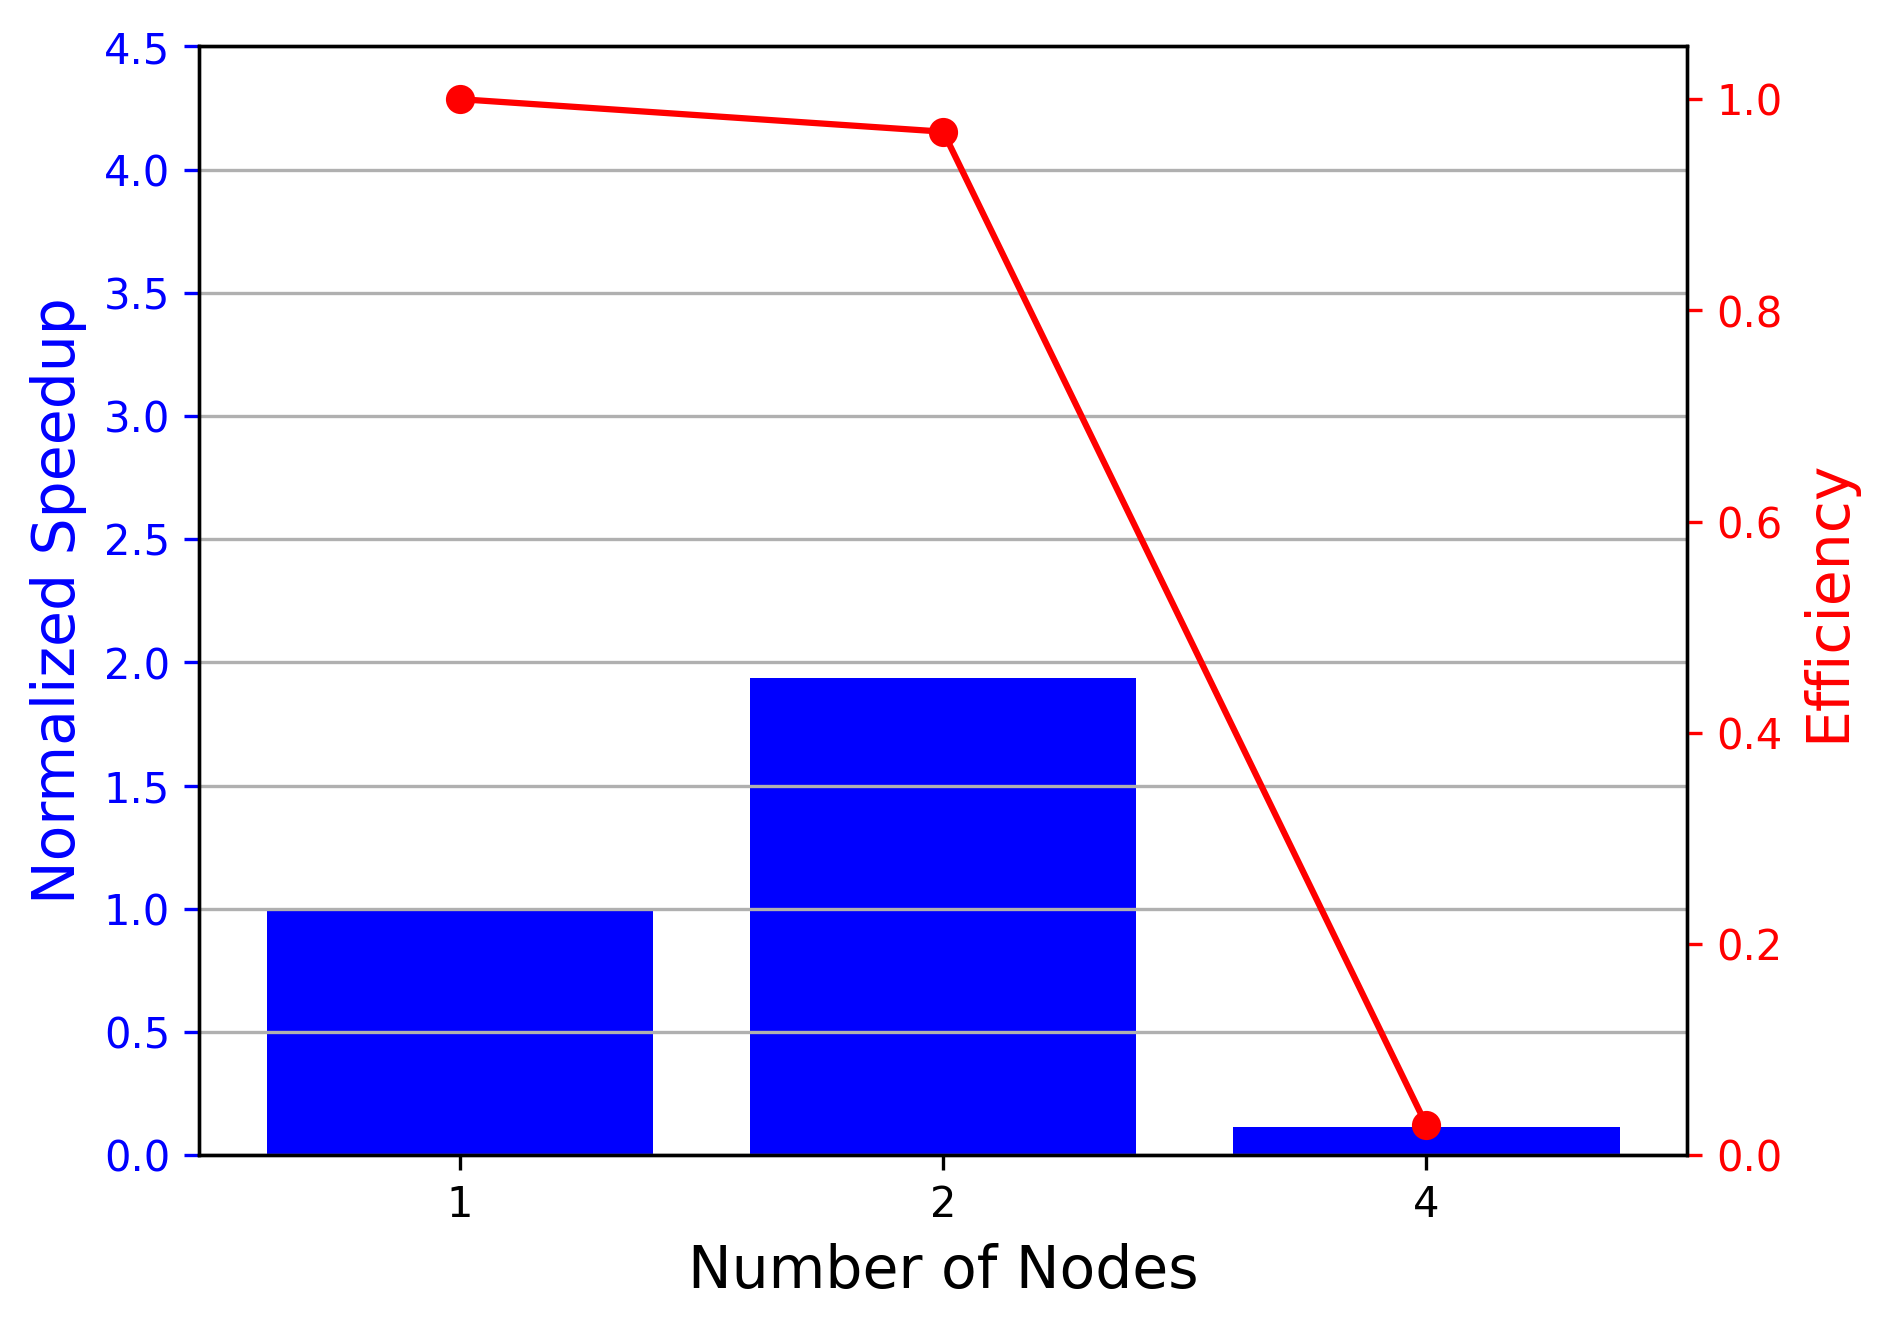
\includegraphics[width=\textwidth,keepaspectratio=true]{../figs/SpeedUp_Eff_COMM.png}
%    \caption{CUDA-Aware-MPI}
%	\label{fig:SpeedEffCpu}
%    \end{subfigure}
%    \caption{Comparison of SpeedUp and Efficiency using CPU+Communication Time As Metric with x, y = 8192 : normal CUDA+MPI vs CUDA-Aware-MPI}
%    \label{figs:Compare4}
%\end{figure}
%- Profiling, bla bla (to see if there are possible improvements)
But, why the CUDA-Aware MPI implementation perform slower than the original CUDA, especially when we have 4 MPI processes? We profiled our implementation with NVIDIA Nsight Systems with the grid size of 512x512. The Listing~\ref{profile1} and ~\ref{profile2} present the profiling results.


\begin{lstlisting}[frame=single,language=bash,caption={Profiling of cuda-aware, gridsize 512 x 512, 2 MPI processes}, label={profile1}, captionpos=b]
 Time(%)  Total Time (ns)           Name    
 -------  ---------------   ---------------------
    76.4        292191744   cudaMallocManaged    
    13.9         53062563   cudaDeviceSynchronize
     4.8         18497584   cudaLaunchKernel    
     1.7          6579209   cudaMemcpyAsync    
 Time(%)  Total Time (ns)              Operation    
 -------  ---------------  ---------------------------------
    47.1          2128041  [CUDA Unified Memory memcpy HtoD]
    39.4          1779778  [CUDA Unified Memory memcpy DtoH]
    13.5           608698  [CUDA memcpy DtoH]   
 Time(%)  Total Time (ns)        Range
 -------  ---------------  -----------------
    44.8        171556950  MPI:MPI_Init
    28.8        110086681  MPI:MPI_Finalize
    15.4         58739812  MPI:MPI_Sendrecv
    11.0         42181167  MPI:MPI_Allreduce
\end{lstlisting}
From Listing~\ref{profile1}, we can see that when we had 2 MPI processes only, \textit{cudaMallocManaged} dominates 76,4\% or 292 milliseconds (ms) which is most of the time spent in CUDA functions, while \textit{cudaDeviceSynchronize} is 13.9\% or 53 ms. But when we had 4 MPI processes (Listing~\ref{profile2}), the most time-consuming function \textit{cuMemcpyAsync} costs 3343 ms while the 2nd one is \textit{cuStreamSynchorize} which is 1395 ms, which were not the case before. In addition, the program also spent a lot of time for \textit{CUDA memcpy} operations instead of \textit{CUDA Unified Memory memcpy}, in total there is around 1000ms for \textit{CUDA memcpy}, while we did not call \textit{CUDA memcpy} anywhere. 

\begin{lstlisting}[frame=single,language=bash,caption={Profiling of cuda-aware, gridsize 512 x 512, 4 MPI processes},label={profile2}, captionpos=b]
 Time(%)  Total Time (ns)          Name    
 -------  ---------------  ---------------------
    62.7       3342704027  cuMemcpyAsync    
    26.2       1394750017  cuStreamSynchronize  
     9.4        499798289  cudaMallocManaged    
     1.1         57059166  cudaDeviceSynchronize
 Time(%)  Total Time (ns)              Operation
 -------  ---------------  ---------------------------------
    52.6        527310844  [CUDA memcpy HtoD]
    46.6        466823849  [CUDA memcpy DtoH]
     0.4          4374463  [CUDA Unified Memory memcpy HtoD]
     0.3          3291129  [CUDA Unified Memory memcpy DtoH]
 Time(%)  Total Time (ns)        Range
 -------  ---------------  -----------------
    92.4       7147306109  MPI:MPI_Sendrecv
     3.7        288412860  MPI:MPI_Init
     2.4        187081352  MPI:MPI_Allreduce
     1.5        115466911  MPI:MPI_Finalize
\end{lstlisting}
\pagebreak
Besides, the time spent for \textit{MPI\_Sendrecv} is 7147 ms which is 121 times higher than with 2 MPI processes. 


To justify for this, let have a look at how the data is send between GPUs. In our case, we have a unified memory implementation, but without GPU Direct support. Everytime we call \textit{MPI\_Sendrecv()}, the hardware/software support unified memory will first check where the data is allocating (in our case it's in GPU since there is a kernel computation before this communication), and then migrate the corresponding pages to correspond CPU, then the CPU send the data to its neighbor MPI processes. The same data migration process is done in the receivers. This implicit memory accessing transfer is not very efficient, results in a big overhead of migrating datas between host and device.

Besides, when we had 4 MPI processes instead of 2 MPI processes, there are ranks which has top/bottom neighbors and they needed to exchange the top/bottom rows which are not memory contiguous due to the column-based data format. Since we used a \textit{MPI\_Type\_Vector} for the MPI communication (check section~\ref{mpi_datatype})), every time we call \textit{MPI\_Sendrecv}, the MPI deamon needs to pack the data which is most likely still in the GPUs. This packing process even got worse when it needs to pack the (top/bottom) rows which are strided data. These packing results in non-coalesced memory accesses which perform badly with GPUs. From the profiling, we can see that this memory access actually call \textit{CUDA memcpy} since it needs to copy data from device to MPI buffer which likely to located on Host. The  non-coalesced caused a huge burden for \textit{CUDA memcpy}, thus resulted in a big spent time. More important, when we accessing data in this manner, it is possible that additional data synchronization is require to make sure data in both gpu and cpu are updated and consistent. The strided data requires to access to more pages, thus causing more overhead to manage those pages. This also explained why in the initial strong scaling test (Figure~\ref{fig:StrongCOMM}), we had very bad performance for 4 MPI processes.

\subsection{Optimization implementations}
In this section, we present our effort to optimize the code. The main works would be first optimizing for the Data accesses for MPI Communication, then try to optimize for data migrations.
\paragraph{Packing/Unpacking data for MPI Communication} Since the strided accesses for exchange ghost layers in row is not very efficient, we decided to implement the packing and unpacking strided data into contiguous data which is used more efficiently by MPI. With this implementation, when we calls \textit{MPI\_Sendrecv}, the MPI deamon only needs to send a contiguous data block which does not create a lot of synchronization and overhead. Besides, we also separated the boundary condition initialization which is implemented in \textit{setBoundaryConditions()} with the synchronization after \textit{exchangeGhostLayer}. Thus the \textit{setGhostLayer()} (which calls \textit{setBoundaryConditions}) is only called once before the time integration loop. With the new implementation, the pseudo code looks like this:

\begin{lstlisting}[frame=single,language=c++, captionpos=b, label={profile3}]
l_waveBlock->setGhostLayer();
while (iteration) // time integration loop
{
	exchangeGhostLayers();
	
	synchGhostLayerAfterWrite(); //data unpacking;
	l_waveBlock->computeNumericalFluxes();
	
	MPI_Allreduce(&l_maxTimeStep, &l_maxTimeGlobal, ...);
	
	l_waveBlock->updateUnknowns(l_maxTimeGlobal);
	synchCopyLayerBeforeRead() // data packing
	
	iteration++;
}
\end{lstlisting}
With this approach, we used 2 household vectors called \textit{topLayer} and \textit{bottomLayer} which allocated on the Unified Memory to store data for communications. The vectors have a size of \textit{6 * row\_size} where the first half \textit{3 * row\_size} are send buffer \textit{h, hv, hu}, the later is for receive buffer. In the packing phase, the GPU kernels copy the according data from the grid to the send buffer, whereas in the unpacking phase GPUs copy the data from the receive buffer back to the grid. Since both buffers are allocated with Unified memory, they can be accessed from both Host and devices. All copy operation happened in device, which are pretty fast. \\
Figure \ref{fig:CompareCudaPacking} shows the improved performance compared to the normal CUDA+MPI version. Compare to our performance in Figure~\ref{figs:Compare2}, packing did boost the performance quite a bit, making our CUDA-Aware version performance came closer to the original CUDA one.
\begin{figure}[htpb]
	\centering
	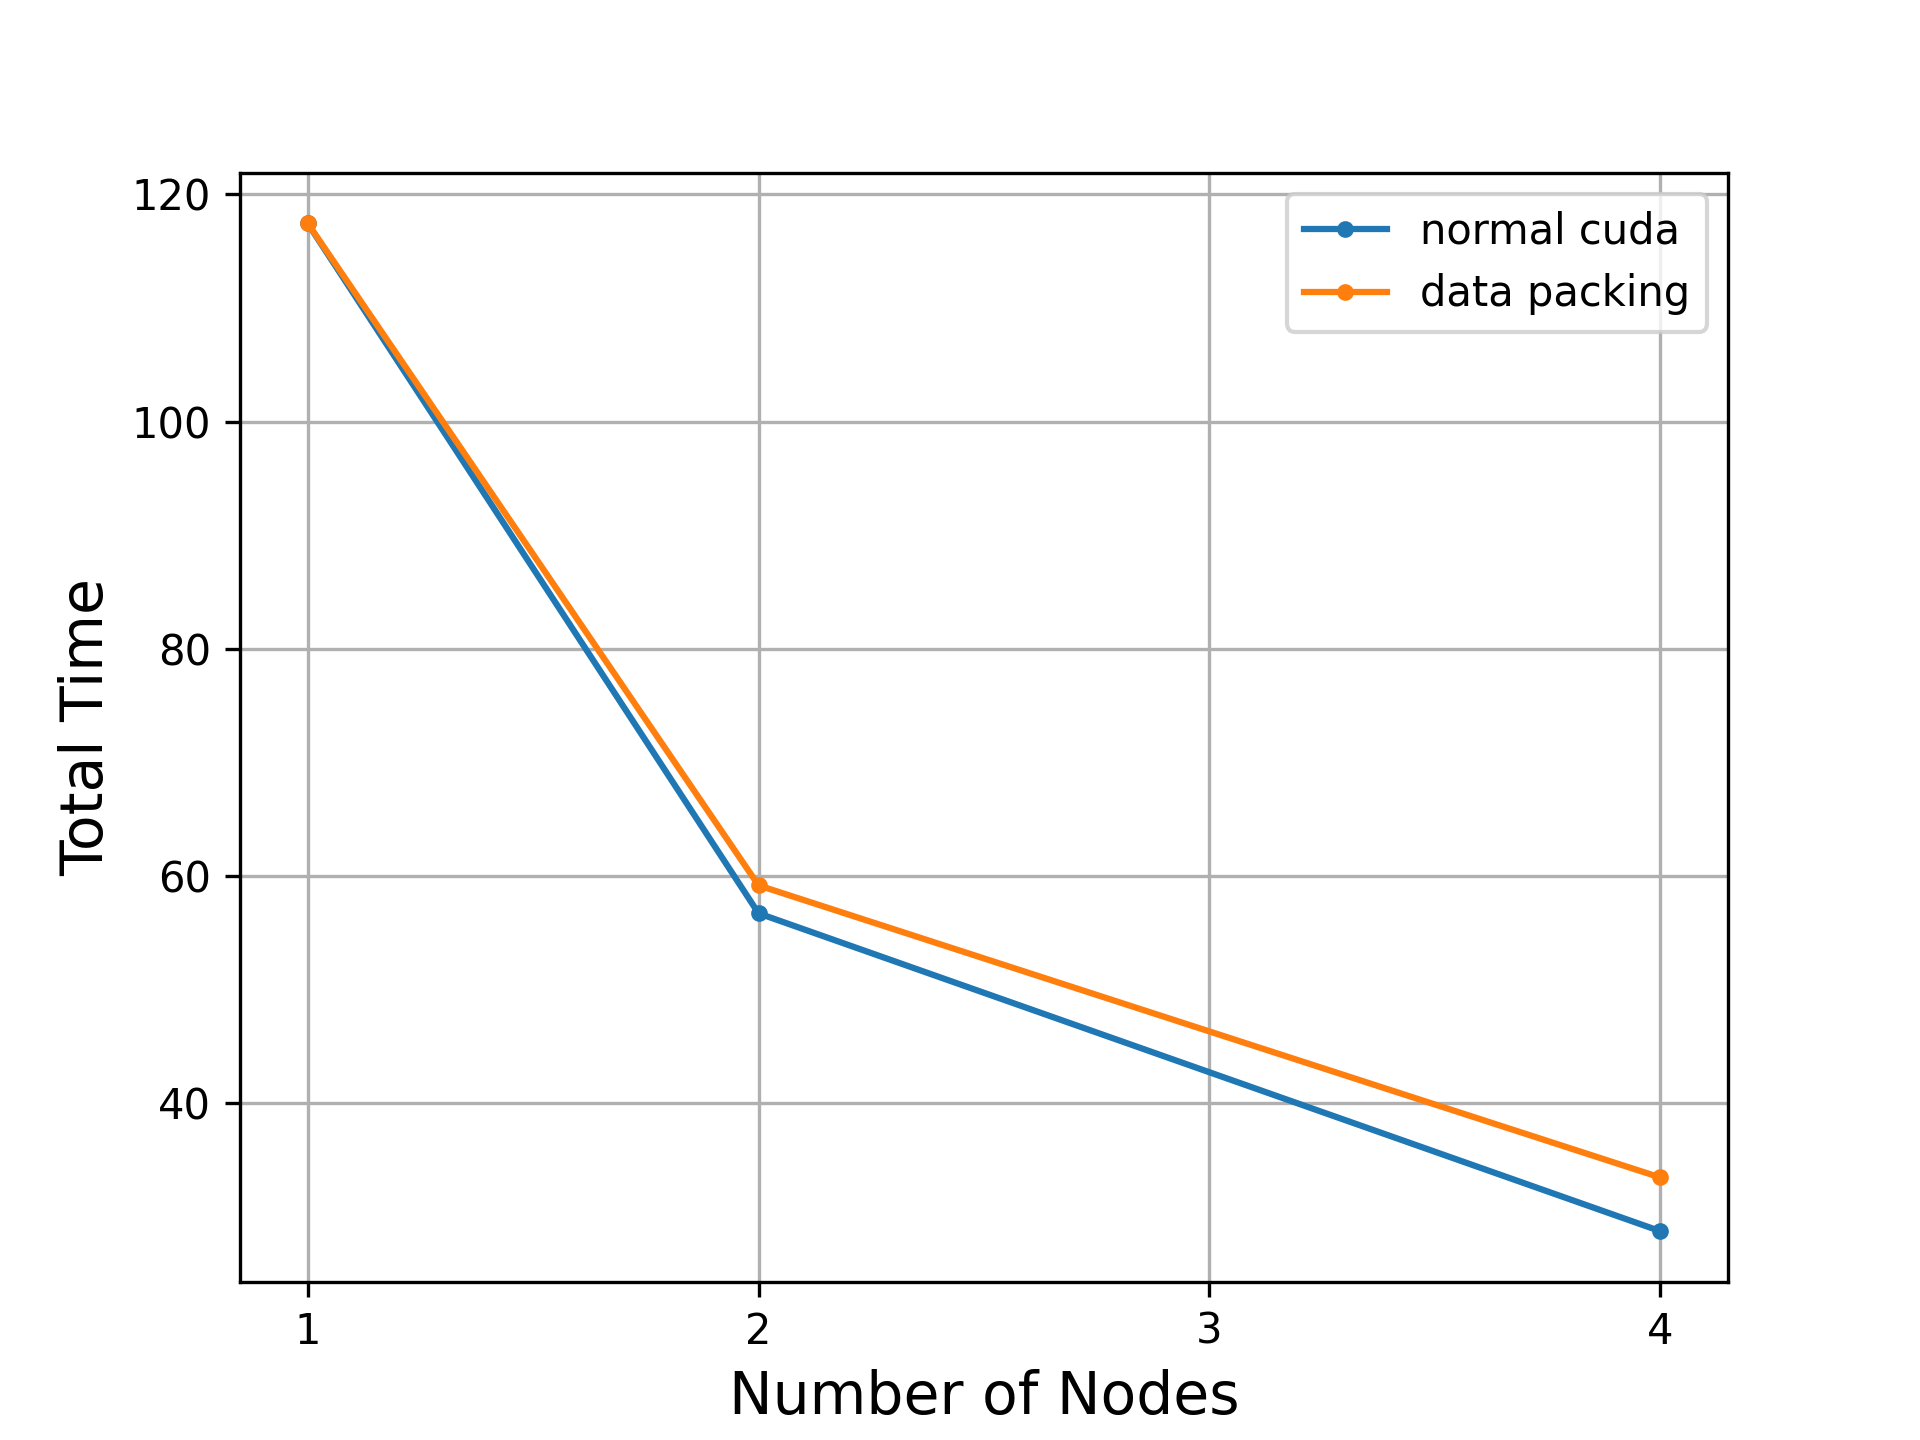
\includegraphics[width=0.7\textwidth,keepaspectratio=true]{../figs/Comparison_CUDA_PACKING.png}
	\caption{Comparison of normal Cuda+MPI and Cuda-Aware-MPI with Data Packing(x,y = 8192) }
	\label{fig:CompareCudaPacking}
\end{figure}

We also had a look at the profiling result in Listing~\ref{profile3}, with packing the program did not spend a lot of time in \textit{cudaDeviceSynchronize} and \textit{cudaMemcpyAsync} anymore, only 56 ms and 6 ms, respectively. Regarding the time for copying data, most of the time spent in \textit{CUDA Unified Memory memcy} which is reasonable, since in our implementation we copied from the grid data to \textit{topLayer} and \textit{bottomLayer} which are both allocated on the Unified Memory. Besides, the time spent for \textit{MPI\_Sendrecv} also improved a lot with packing, it's ~121 ms (without packing it's 7147 ms). The packing technique actually helped to lift a lot of bottlenecks of the initial implementation.
\pagebreak
\begin{lstlisting}[frame=single,language=bash,caption={Profiling of cuda-aware with Packing, gridsize 512 x 512, 4 MPI processes},label={profile3}, captionpos=b]
 Time(%)  Total Time (ns)          Name
 -------  ---------------  ---------------------
    84.9        497957591  cudaMallocManaged
     9.6         56439841  cudaDeviceSynchronize
     2.5         14836003  cudaLaunchKernel
     1.0          6130341  cudaMemcpyAsync
 Time(%)  Total Time (ns)              Operation
 -------  ---------------  ---------------------------------
    50.7          2216590  [CUDA Unified Memory memcpy HtoD]
    36.5          1596835  [CUDA Unified Memory memcpy DtoH]
    12.7           555683  [CUDA memcpy DtoH]
 Time(%)  Total Time (ns)        Range
 -------  ---------------  -----------------
    50.8        251692211  MPI:MPI_Init
    24.6        121808411  MPI:MPI_Sendrecv
    18.3         90864549  MPI:MPI_Finalize
     6.3         30970963  MPI:MPI_Allreduce
\end{lstlisting}
%PUT FIGURE HERE
% WRITE SOMETHING ABOUT THE RESULT

\paragraph{Data Migration Optimization}
Accoriding to \cite{unifiedMemory}, On GPUs, managed memory may not be physically allocated when cudaMallocManaged() returns; 
it may only be populated on access (or prefetching). In other words, pages and page table entries may not be created until they are accessed by the GPU or the CPU. 
The pages can migrate to any processor's memory at any time, and the driver employs heuristics to maintain data locality and prevent excessive page faults.


In a real application, the GPU is likely to perform a lot more computation on data (perhaps many times) without the CPU touching it. In our case, the computations are mostly done inside
the kernel function computeNetUpdatesKernel() and updateUnknownsKernel().
There are a few different ways that we can eliminate or change the migration overhead 
\begin{figure}[htpb]
	\centering
	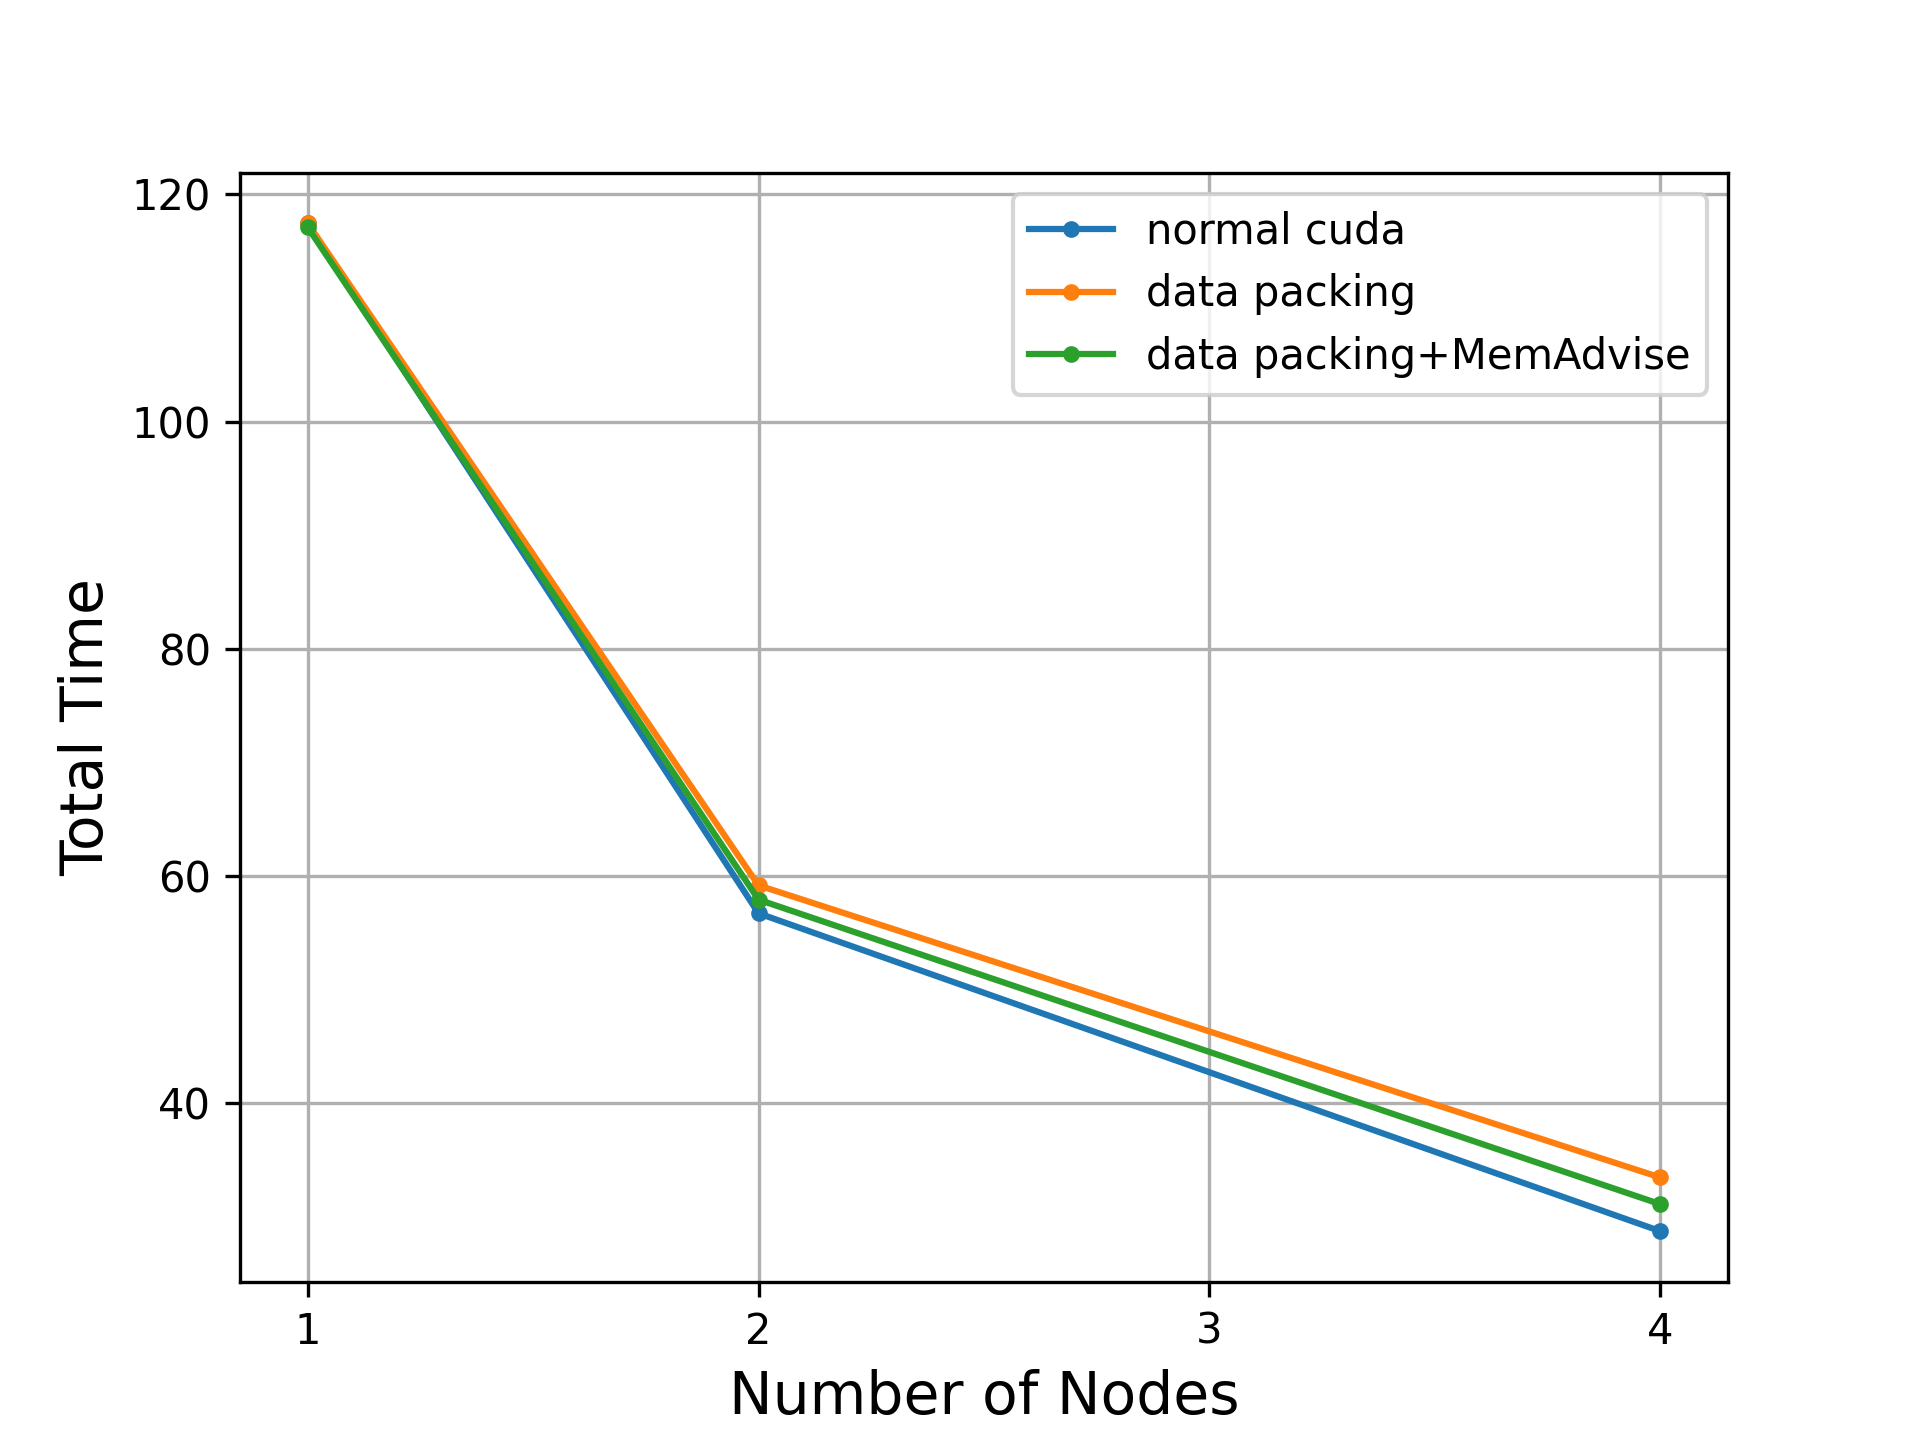
\includegraphics[width=0.7\textwidth,keepaspectratio=true]{../figs/Comparison_CUDA_PACKING_MemAdvise.png}
	\caption{normal Cuda+MPI Vs. Cuda-Aware-MPI with Data Packing Vs. Cuda-Aware-MPI with Data Packing and MemAdvise (x,y = 8192) }
	\label{fig:CompareCudaPackingMem}
\end{figure}

\begin{itemize}
    \item  Move the data initialization to the GPU in another CUDA kernel. 
	Which is implemented in \textit{SWE\_BlockCudaAwareMPI::initScenario()} function. 
	Use \\
	\textit{-DENABLE\_CUDA\_OPT\_INIT} option of cmake to play around with this feature. (Since the data will be copied between CPU and GPU multiple times during the runtime of our program, this won't help too much)
\end{itemize}

\begin{itemize}
	% \item \textit{cudaMallocManaged}: \textit{GlobalMemAttachGlobal} means just initialization, not allocation yet.
	% \item \textit{initScenario}: allocate on GPUs
	\item In \textit{exchangeGhostLayers} function, we use \textit{cudaMemAdvise} to guide the driver about where to migrate the data.
	There are two options we can set: 
		\begin{itemize}
			\item \textit{cudaMemAdviseSetPreferredLocation}
				% For sendbuf: \\ % Assume that 2 GPUs can talk directly through PCIe
			% 	\textit{cudaMemAdvise(data, N, ..SetReadMostly, gpuId)}; \\
			%  	\textit{cudaMemPrefetchAsync(data, N, gpuId, s)};\\
			%   	\textit{cudaMemAdviceUnsetReadMostly}
			\item \textit{cudaMemAdviseSetAccessedBy}
			%  Recvbuf: 
			%  \textit{cudaMemAdvise(data, N, ..PreferredLocation, gpuId);}
	\end{itemize}
	We tried with both options and find that \textit{cudaMemAdviseSetPreferredLocation} gives us a better performance. Regarding where to migrate the data, we set it as \textit{cudaCpuDeviceId} which means the data should be migrated to hosts and it did boost the performance. This is reasonable, since we did not have GPUDirect, then all communications need to go through host. This hint helps the MPI to locate and pack data effectively. \\
	
	\item We also tried to use \textit{MemAdvise} for \textit{computeNetFluxes} and \textit{updateUnknowns}, but it turned out that using \textit{MemAdvise} inside these two functions not only could not boost the performance, but also might slow down the program. Moreover, the explicit fetching the data by using \textit{cudaMemPrefetchAsync} also did not help the performance. We guess that because we had "First touch" implementation in the \textit{initScenario} which made data already located on GPUs, thus further hints are not needed.  
	% \item \textit{computeNetFluxes}: \\
	% 		\textit{cudaMemAdvise(data, N, ..SetReadMostly, gpuId)}; \\
	% 		\textit{cudaMemPrefetchAsync(data, N, gpuId, s)};\\
	% \item \textit{updateUnknowns}:
	% 		\textit{cudaMemAdvise(data, N, ..PreferredLocation, gpuId);}
\end{itemize}

Figure \ref{fig:CompareCudaPackingMem} shows the further improved performance of the CUDA-Aware MPI compared to previous one as well as the original cuda implementation. As we can see, the optimization for data migration made the performance slightly faster for this test case. This also helps the performance line of CUDA-Aware MPI comes closer to the tradition CUDA approach, even though it is still slightly slower but not significantly slower.


\paragraph{Non-Blocking MPI Routines}
We also tried to replace the \textit{MPI\_Sendrecv} with non-blocking routines (\textit{MPI\_Isend} and \textit{MPI\_Irecv}) so that we can overlap those send and recv operations and possible some computations. The overlapping communication and computation did speed up the performance, however, resulted in some small silenced errors (only detected with \textit{error\_check.py}). Thus, we would not submit this version. Insteads, we have a pure overlapping communications(no overlapping with computations), where \textit{MPI\_Waitall} were called after all \textit{MPI\_Isend} and \textit{MPI\_Irecv} are called. \\

The result are presented in figure \ref{fig:CompareCudaPackingMemNonBlock}, where the Non-blocking implementation improves the performance of CUDA-Aware MPI, make it as fast as the traditional CUDA. Even though this is not an fair-comparison since the original CUDA implementation was with Blocking communications, this shown our efforts to optimize the code.
\begin{figure}[htpb]
	\centering
	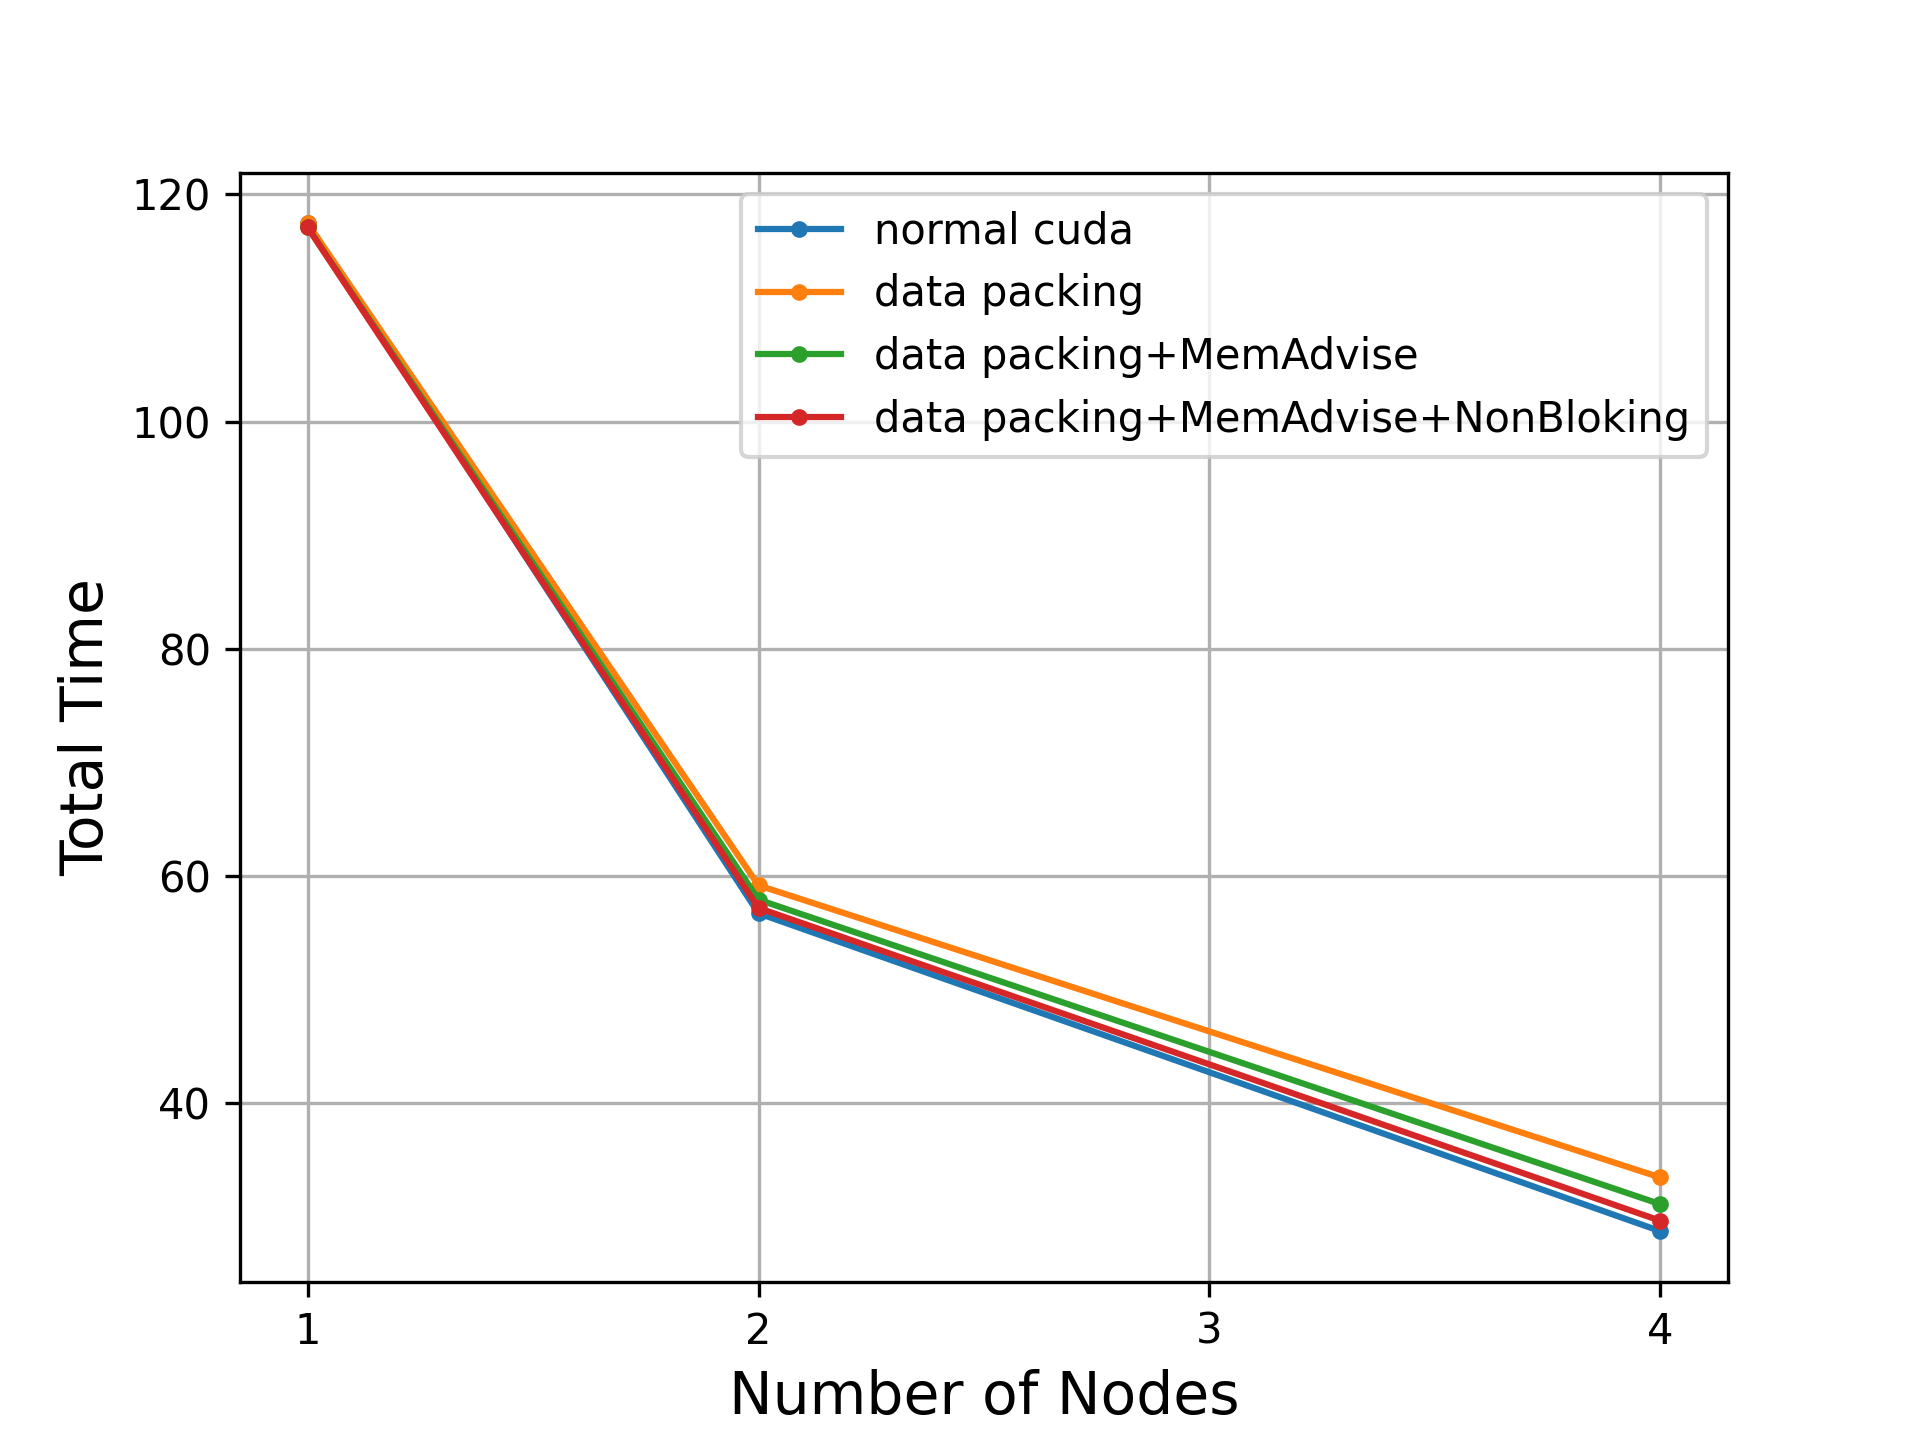
\includegraphics[width=0.7\textwidth,keepaspectratio=true]{../figs/Comparison_CUDA_PACKING_MemAdvise_NonBlocking.png}
	\caption{Comparison of all optimizations(x,y = 8192) }
	\label{fig:CompareCudaPackingMemNonBlock}
\end{figure}

%\subsection{Optimization at Runtime + Profiling}
%+ Comparison between with and without GPUDirect
%+ Comparison between with GPUDirect P2P vs RDMA
%+ Profiling (to explain what happens in these different modes, check the slide).
\paragraph{Optimizations at runtime}
Due to limitation of the test system, we could not test our implementation with a GPU Direct RDMA nor with MPS, nor GPU Direct P2P.   

\subsection{Future works}
Possible future works are:
\begin{itemize}
	\item Testing the implementation with different Runtime optimization: GPU Direct RMDA, GPU Direct P2P, MPS.
	\item Overlapping Computations with Communications.
\end{itemize}

\subsection{Final Result}
Finally, we chose the best optimized version, which as shown in figure \ref{fig:CompareCudaPackingMemNonBlock},
is the one with all optimization features, to compare the SpeedUp and the Efficiency.
We see from figure \ref{fig:final} that both normal cuda+mpi and cuda-aware-mpi scaled quite well. With 2 GPU nodes, we observe a speedup over 2(super scaling).
Possible reason can be that with 2 GPUs we have higher bandwidth and thus achieved a better performance. Or perhaps the smaller block somehow fits better to the GPU memory and thus can be loaded more efficiently.
When it scales to 4 GPU nodes, our cuda-aware-mpi version looks a bit slower than the normal cuda+mpi one, but still really close to 4 times SpeedUp.
\begin{figure}[htpb]
    \centering
    \begin{subfigure}{.4\textwidth}
        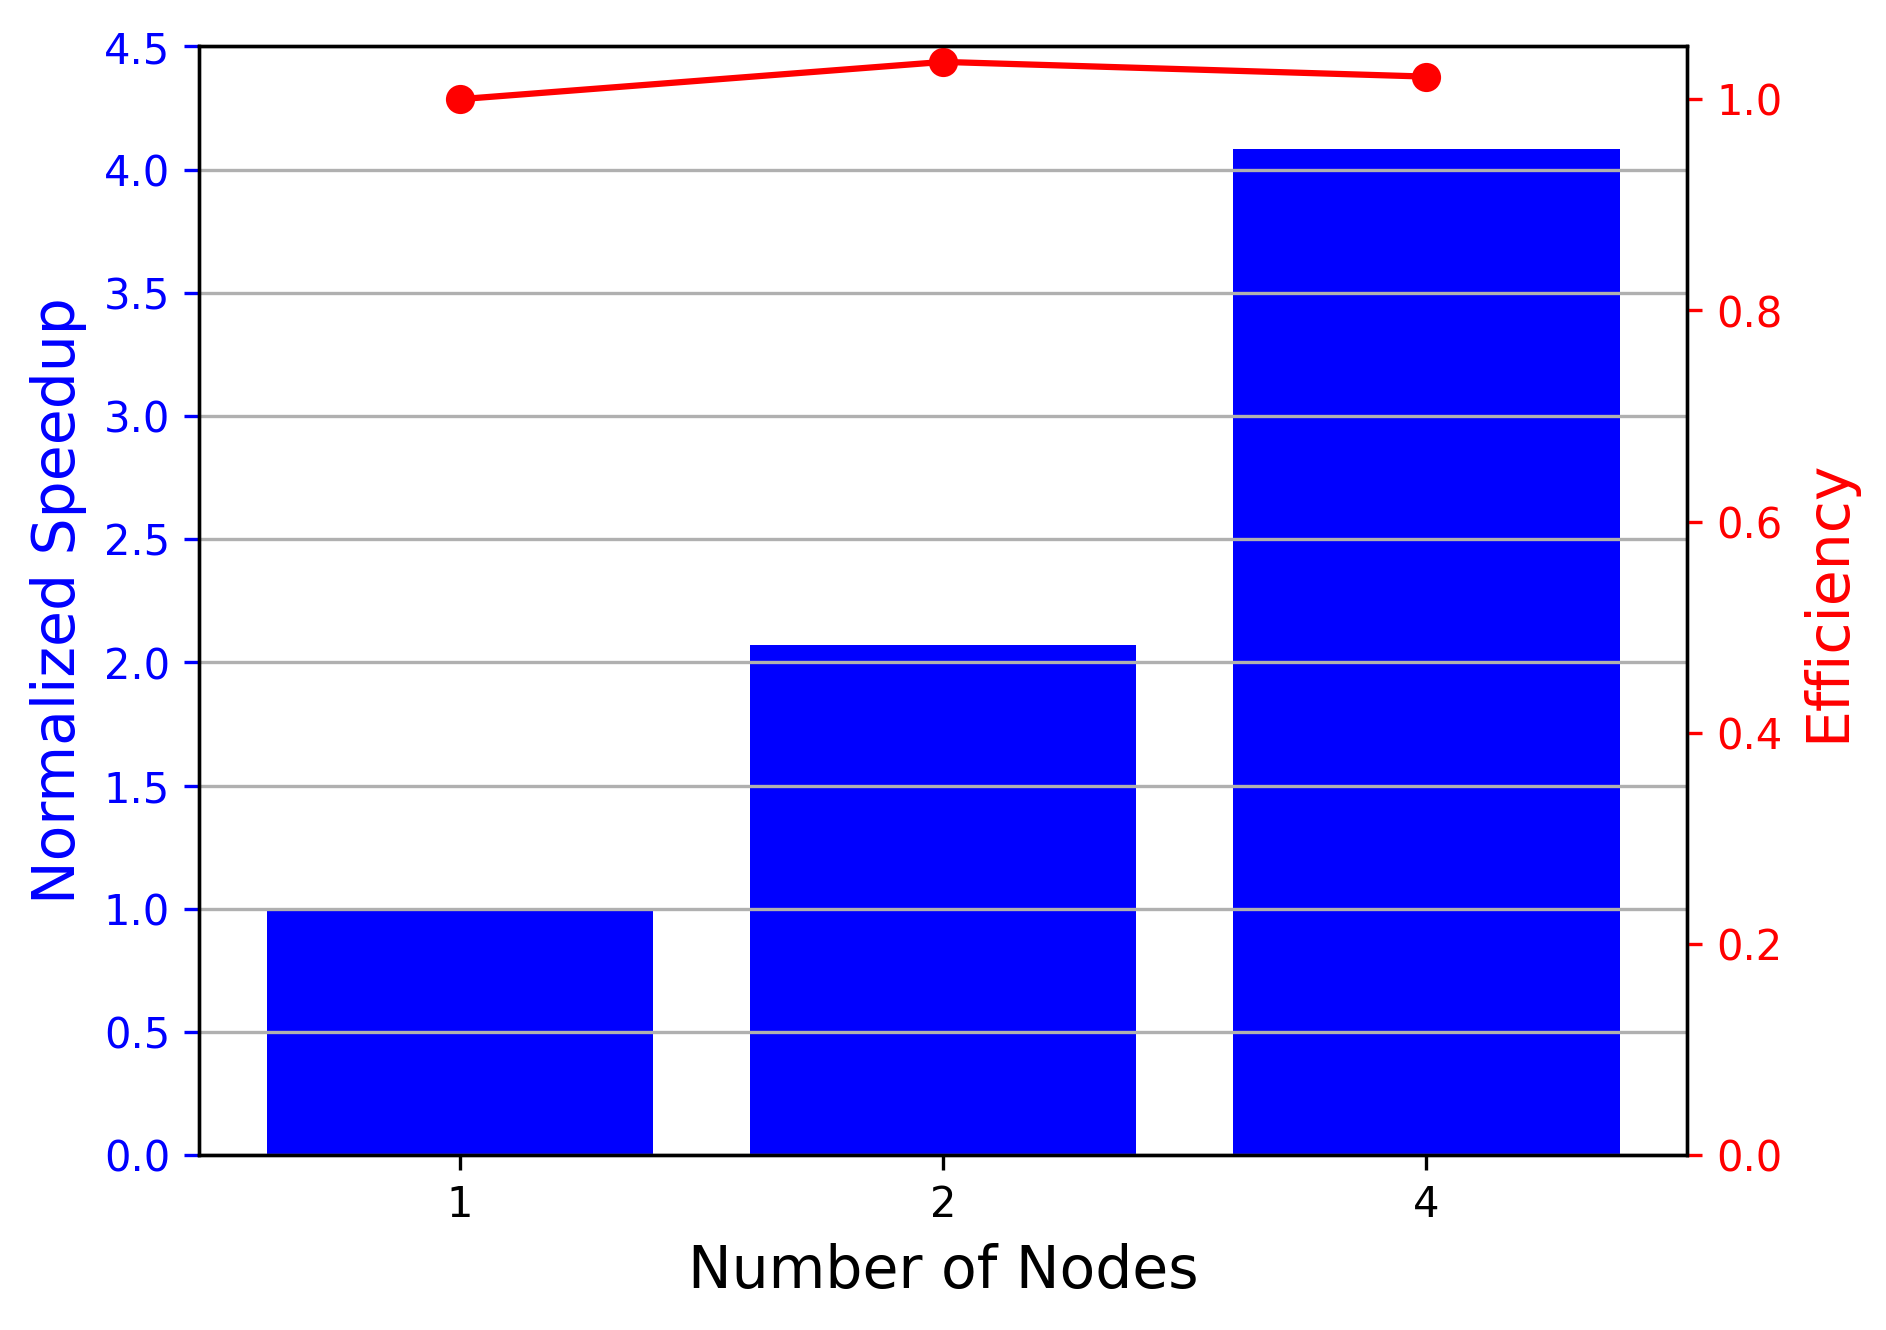
\includegraphics[width=\textwidth,keepaspectratio=true]{../figs/SpeedUp_Eff_COMM_CUDA.png}
        \caption{normal cuda+mpi}
        \label{fig:finalcuda}
    \end{subfigure}
%
    \begin{subfigure}{.4\textwidth}
    	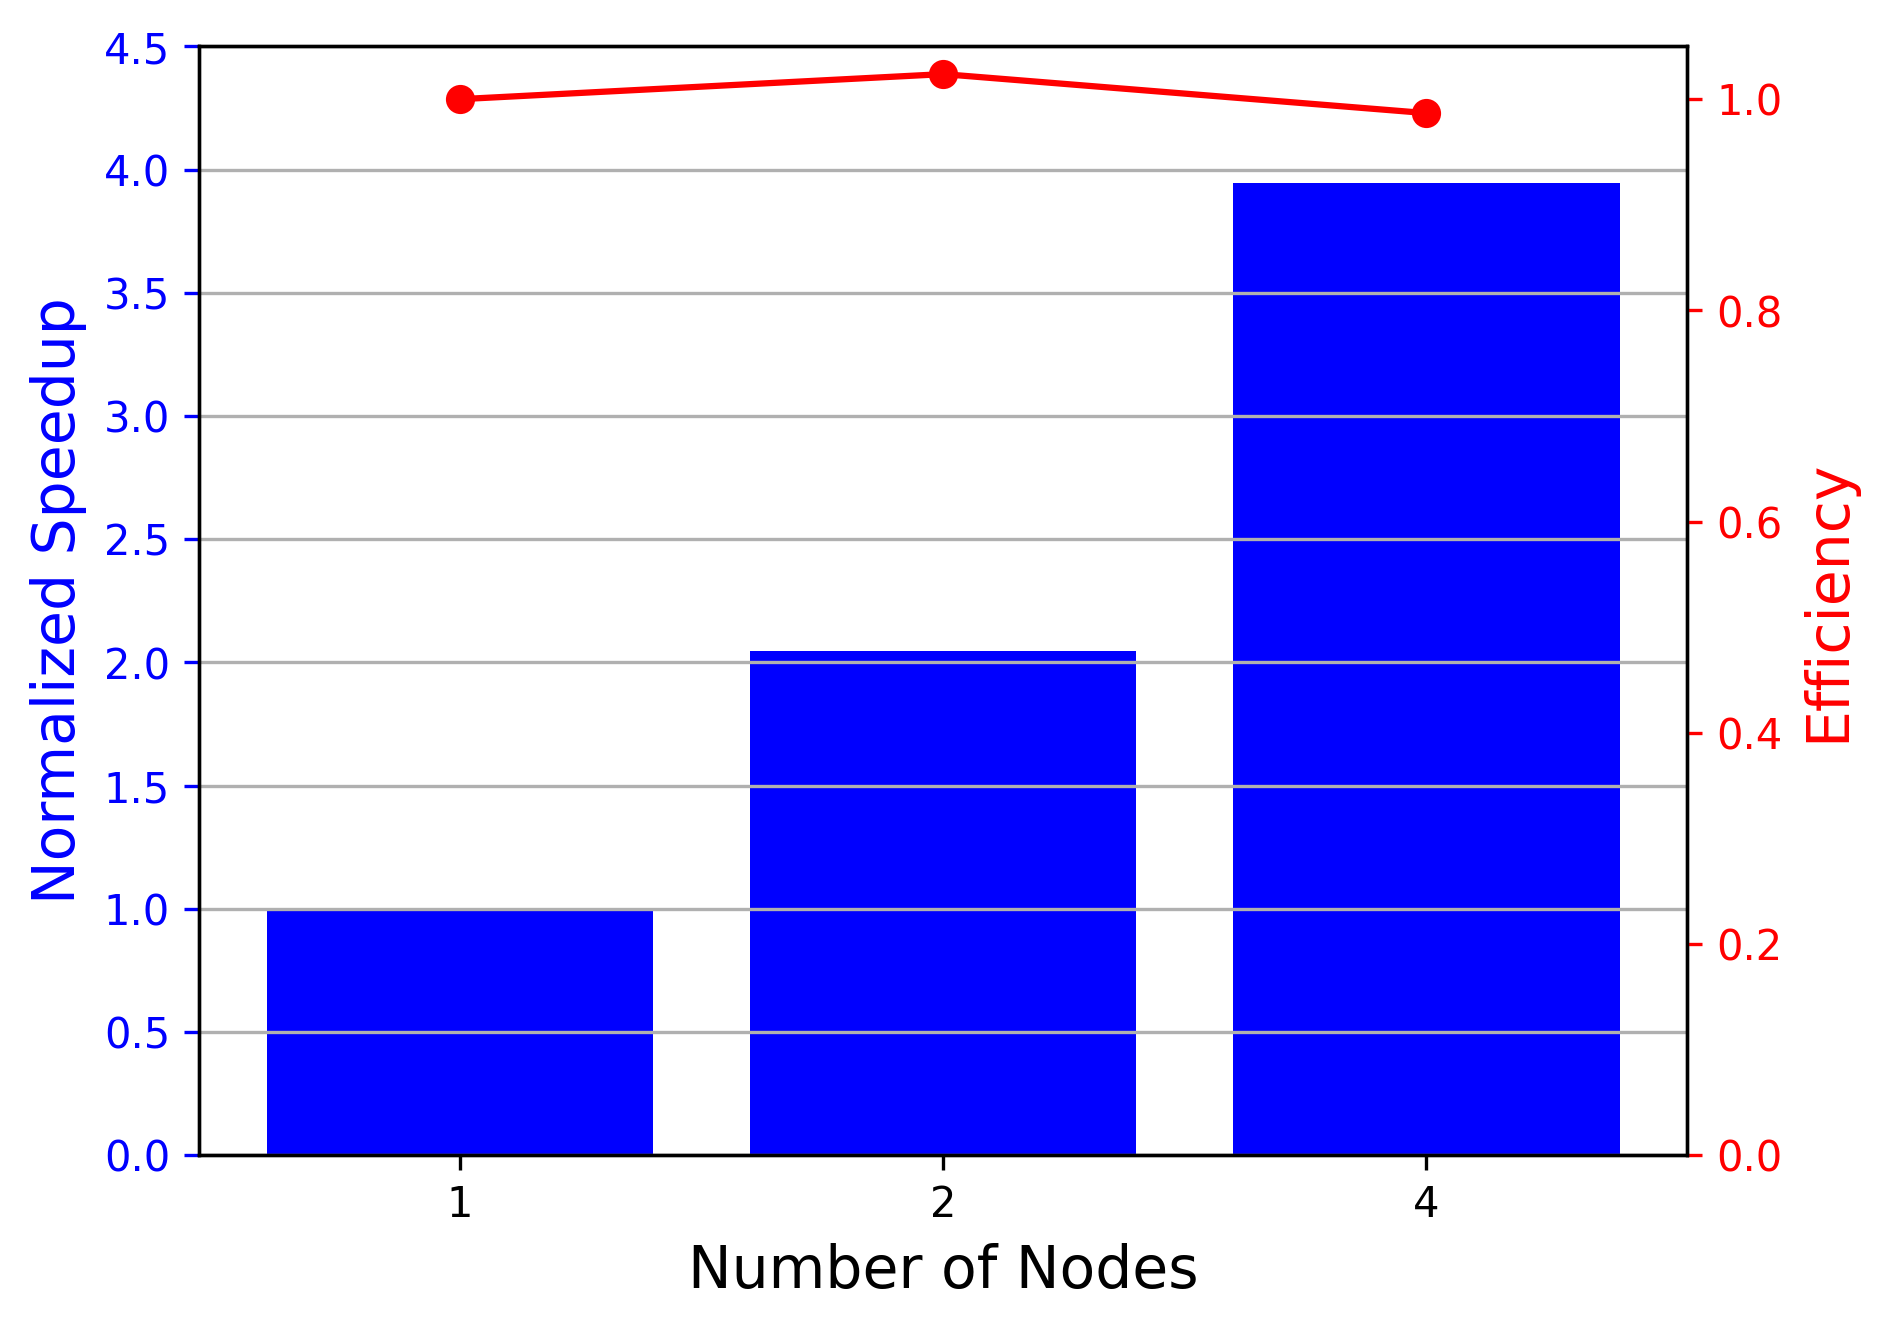
\includegraphics[width=\textwidth,keepaspectratio=true]{../figs/final_optimized.png}
    	\caption{final optimized cuda-aware-mpi}
    	\label{fig:finalcudaAware}
    \end{subfigure}
	\caption{Comparison of the Efficiency and Speedup(x,y = 8192): normal CUDA+MPI Vs. Cuda-Aware-MPI}
	\label{fig:final}
\end{figure}

\section{Conclusion}
In conclusion, we successfully implemented CUDA-Aware MPI for the SWE code with Virtual Unified Memory and the implementation worked correctly. Besides, we also found and fixed some minor bugs in the original CUDA implementation. However, due to the limitation of the testing system, the advantage of CUDA-Aware MPI could not be exploited. But without GPU Direct support, we managed to make our code works almost as fast as the original CUDA, and as correct as the original one. Besides, given the current development of CUDA, we learned that Virtual Unified Memory can give as good performance as the traditional approach where data allocated on host and device separatedly and additional moving data step are required. With that, using Virtual Unified Memory is much easier to handle.
\\
\\
We have learned a lot about GPUs and GPU Programming in general, and CUDA in particular.    


\medskip
%\printbibliography
\bibliography{myref}{}
\bibliographystyle{plain}

\end{document}


